  %%
  %% Copyright 2007-2025 Elsevier Ltd
  %%
  %% This file is part of the 'Elsarticle Bundle'.
  %% ---------------------------------------------
  %%
  %% It may be distributed under the conditions of the LaTeX Project Public
  %% License, either version 1.3 of this license or (at your option) any
  %% later version.  The latest version of this license is in
  %%    http://www.latex-project.org/lppl.txt
  %% and version 1.3 or later is part of all distributions of LaTeX
  %% version 1999/12/01 or later.
  %%
  %% The list of all files belonging to the 'Elsarticle Bundle' is
  %% given in the file `manifest.txt'.
  %%
  %% Template article for Elsevier's document class `elsarticle'
  %% with Harvard-style bibliographic references

  \documentclass[preprint,12pt,numbers]{elsarticle}
  %% Use the option review to obtain double line spacing
  %% \documentclass[authoryear,preprint,review,12pt]{elsarticle}

  %% Use the options 1p,twocolumn; 3p; 3p,twocolumn; 5p; or 5p,twocolumn
  %% for a journal layout:
  %% \documentclass[final,1p,times,authoryear]{elsarticle}
  %% \documentclass[final,1p,times,twocolumn,authoryear]{elsarticle}
  %% \documentclass[final,3p,times,authoryear]{elsarticle}
  %% \documentclass[final,3p,times,twocolumn,authoryear]{elsarticle}
  %% \documentclass[final,5p,times,authoryear]{elsarticle}
  %% \documentclass[final,5p,times,twocolumn,authoryear]{elsarticle}

  %% For including figures, graphicx.sty has been loaded in
  %% elsarticle.cls. If you prefer to use the old commands
  %% please give \usepackage{epsfig}

  %% The amssymb package provides various useful mathematical symbols
  \usepackage{amssymb}
  %% The amsmath package provides various useful equation environments.
  \usepackage{amsmath}
  \usepackage{siunitx}
  \usepackage{enumitem}   % for enumerate with custom labels (roman numerals)
  \usepackage{xcolor}
  %% \todo{...} marks places where Amirali must supply a real value / detail.
  %% Search the source for "TODO" to find every gap before submission.
  \newcommand{\todo}[1]{\textcolor{red}{\textbf{[TODO: #1]}}}
  \newcommand{\repourl}{https://github.com/AmiraliKhosrozadeh/ice-bonded-granular-microCT}
  %% The amsthm package provides extended theorem environments
  %% \usepackage{amsthm}

  %% For subfigures
  \usepackage{subcaption}

  %% For rotating tables
  \usepackage{rotating}
  \usepackage{pdflscape}
  \usepackage{multirow}
  \usepackage{booktabs}
  %% Suppress the /PTEX.* private keys that pdfTeX writes into the output for
  %% every included PDF figure (source filename, page number, info dict).  They
  %% are non-standard keys, some submission systems and PDF/A validators flag
  %% them, and they serve no purpose in a finished document.  This is a pdfTeX
  %% primitive, not a post-processing step, so the PDF is clean as produced.
  \ifdefined\pdfsuppressptexinfo\pdfsuppressptexinfo=-1\fi   % \toprule/\midrule/\cmidrule (also needed by specimen_table.tex)
  \usepackage{url}
  \urlstyle{same}   % the address in the running font, not typewriter
  \usepackage{longtable}
  \usepackage{array}

  %% For flowcharts
  \usepackage{tikz}
  \usetikzlibrary{shapes.geometric, arrows.meta, positioning, fit, backgrounds}

  %% The lineno packages adds line numbers. Start line numbering with
  %% \begin{linenumbers}, end it with \end{linenumbers}. Or switch it on
  %% for the whole article with \linenumbers.
  \usepackage{lineno}

  \journal{}

  \begin{document}

  \begin{frontmatter}

  %% Title, authors and addresses

  \title{Grain-scale kinematics, ice-bond failure and damage evolution in
         ice-bonded granular media under in-situ uniaxial
         compression} %% Article title

  %% use optional labels to link authors explicitly to addresses:
  \author[inst1]{Amirali Khosrozadeh\corref{cor1}}
  \ead{amirali.khosrozadeh@tuhh.de}
  \cortext[cor1]{Corresponding author}
  \author[inst2]{Yannik Sinnwell}
  \author[inst1]{Swantje Pietsch-Braune}
  \author[inst2]{Kai Nikolaus}
  \author[inst2]{Sergiy Antonyuk}
  \author[inst1]{Stefan Heinrich}

  %% Author affiliations
  \affiliation[inst1]{organization={Institute of Solids Process Engineering
              and Particle Technology, Hamburg University of Technology},%
              addressline={Denickestrasse 15},
              city={Hamburg},
              postcode={21073},
              country={Germany}}

  \affiliation[inst2]{organization={Institute of Particle Process Engineering,
              University of Kaiserslautern-Landau (RPTU)},%
              addressline={Gottlieb-Daimler-Stra{\ss}e 44},
              city={Kaiserslautern},
              postcode={67633},
              country={Germany}}

  %% Abstract
  \begin{abstract}
  Bonded-particle models of frozen particle systems rest on grain-scale
  quantities that are at present assumed rather than measured, namely how the ice
  bridges between grains are arranged, where those bridges fail, and how a
  packing loses them as it is loaded.  This study images the interior of ice-bonded
  granular columns while they are being compressed, by combining in-situ
  cryogenic uniaxial compression at $-5\,^\circ$C with micro-computed
  tomography, so that the same specimen is reconstructed at every load step.
  Twelve specimens spanning spherical glass beads, angular $\gamma$-alumina and
  natural quartz sand are analysed for grain kinematics, for the ice-bond
  network and its failure modes, for the damage that develops, and for the
  evolving transport properties of the pore and ice networks.  The ice bridges
  are found to fail both through their own thickness and at the grain--ice
  interface.  At the reference threshold the crack comes within the
  \SI{114}{\micro\meter} the scan can resolve of at least one interface in
  $85\%$ of the 431 cracked bridges, and in about half of them that face has
  lost at least half its ice, so the common mode is mixed, interfacial over
  part of the bridge and through the ice over the rest, and a clean
  interfacial break was resolved once.  Bonds are lost predominantly by
  separation as the packing dilates rather than by rupture in place, so the
  broken fraction is not a measure of bond strength.  Cracking initiates at the
  unconfined lateral surface and progresses inward without organising into a
  planar feature, and the sand accommodates shortening by compaction and then
  flow rather than by fracture.  Each condition was tested on a single
  specimen, so the reported variability is spatial rather than between
  specimens.
  \end{abstract}

  %% Graphical abstract
  %\begin{graphicalabstract}
  %\includegraphics[width=\linewidth]{figures/graphical_abstract.png}
  %\end{graphicalabstract}

  %% Research highlights
  \begin{highlights}
  \item Cryogenic in-situ rig re-images the same frozen specimen at successive load steps
  \item Bonds are lost by separation as the packing dilates, not by rupture in place
  \item Most ice bridges fail in mixed mode, along a grain face and then through the ice
  \item Cracking starts at the free surface and never organises into a plane
  \end{highlights}

  %% Keywords
  \begin{keyword}
  In-situ micro-computed tomography \sep
  Ice-bonded granular material \sep
  Ice-bond failure \sep
  Grain-scale kinematics \sep
  Digital volume correlation \sep
  Uniaxial compression \sep
  Deep-learning instance segmentation
  \end{keyword}

  \end{frontmatter}

  % \linenumbers

  %% main text
  %%

  \section*{Nomenclature}
  \setlength{\LTleft}{0pt}\setlength{\LTright}{\fill}
  \begin{longtable}{@{}p{0.21\textwidth}p{0.73\textwidth}@{}}
  \hline
  \multicolumn{2}{@{}l}{\textit{Specimen and microstructure}}\\
  $A_0$ & Specimen cross-sectional area at the first scan \\
  $d_0$, $h_0$ & Specimen diameter and height at the first scan \\
  $n_\mathrm{scan}$ & Number of CT scans of the specimen \\
  $D_{10}, D_{50}, D_{90}$ & Percentiles of the volume-weighted size distribution \\
  $q_3$, $Q_3$ & Incremental and cumulative volume-weighted size distribution \\
  $S_a$ & Mean areal roughness parameter of the bead surface \\
  $V_\mathrm{air}$, $V_\mathrm{ice}$, $V_\mathrm{grain}$ & Volume of the air, ice and grain phases \\
  $V_\mathrm{interior}$ & Specimen interior volume, $V_\mathrm{air}+V_\mathrm{ice}+V_\mathrm{grain}$ \\
  $\phi_\mathrm{ice}$ & Ice volume fraction of the specimen interior \\
  $\rho$ & Particle packing fraction \\
  $S$ & Degree of ice saturation, $\phi_\mathrm{ice}/(1-\rho)$ \\
  $\varepsilon$ & Porosity, the air-class volume fraction of the interior \\
  $S_V$ & Specific surface of the air--solid interface \\
  $\tau_\mathrm{ice}$ & Tortuosity of the ice network \\
  $k$ & Kozeny--Carman permeability \\
  $k_K$ & Kozeny constant, 5 in the Carman form of Eq.~\eqref{eq:kc} \\
  $E_\mathrm{eq}$ & Equivalent (deviatoric) Green--Lagrange strain, Eq.~\eqref{eq:eqstrain} \\
  $D_{\mathrm{eff},z}$ & Effective axial diffusivity of the ice phase, $D_0 = 1$ \\
  $z$ & Coordination number of a grain \\
  \hline
  \multicolumn{2}{@{}l}{\textit{Grain kinematics and strain}}\\
  $\mathbf{x}_i$, $\mathbf{u}_i$ & Reference position and displacement of grain $i$ \\
  $\mathcal{N}(i)$ & Set of the 16 nearest neighbours of grain $i$ \\
  $\mathbf{G}$, $\mathbf{c}$ & Fitted displacement gradient and constant offset \\
  $\mathbf{F}$, $\mathbf{I}$ & Deformation gradient and identity tensor \\
  $\mathbf{E}$ & Green--Lagrange strain tensor \\
  $E_{zz}$ & Axial Green--Lagrange strain \\
  $F_{zz}$ & Axial stretch, $L_B/L_A$ \\
  $L_A$, $L_B$ & Column length measured in the two scans \\
  $p_z$ & Height of a grain in the reference scan \\
  $\Phi$, $\|\Delta\Phi\|$ & Affine transformation returned by the correlation, and its incremental norm \\
  $u_r/r$ & Radial displacement normalised by radial position \\
  \hline
  \multicolumn{2}{@{}l}{\textit{Ice bonds and their failure}}\\
  $A$, $B$ & The two grains of a bonded pair \\
  $d_A$, $d_B$ & Distance from a voxel to the surface of grain $A$ or $B$ \\
  $g$ & Free gap between the two grain surfaces \\
  $s$ & Slack setting the footprint radius of the throat lens \\
  $r_i$, $r_j$ & Radii of two grains \\
  $q$ & Position of a crack across a throat, $0$ at a grain surface and $0.5$ at mid-bond \\
  $c_A$, $c_B$ & Ice coverage remaining on each of the two grain faces \\
  $c_\mathrm{hi}$, $c_\mathrm{lo}$ & Larger and smaller of $c_A$ and $c_B$ \\
  $C_\mathrm{HI}$, $C_\mathrm{LO}$ & Coverage thresholds of the failure-mode classification \\
  $\alpha_b$ & Broken fraction of the followed bonds \\
  \hline
  \multicolumn{2}{@{}l}{\textit{Damage and its spatial organisation}}\\
  $d$ & Grain diameter, as the unit of the clustering neighbourhood \\
  $R_\mathrm{nb}$ & Neighbourhood radius of the breakage-event clustering \\
  $\lambda_2$, $\lambda_3$ & Second and third eigenvalues of a damage component point cloud \\
  \hline
  \multicolumn{2}{@{}l}{\textit{Abbreviations}}\\
  BPM & Bonded-particle model \\
  CT & Computed tomography \\
  DBSCAN & Density-based spatial clustering of applications with noise \\
  DDIC & Discrete digital volume correlation \\
  DEM & Discrete element method \\
  DVC & Digital volume correlation \\
  EDT & Euclidean distance transform \\
  HR & High roughness, the abraded glass beads \\
  LDIC & Local digital volume correlation \\
  PFS & Particle-fluid system \\
  PMMA & Poly(methyl methacrylate) \\
  PSD & Particle-size distribution \\
  PuMA & Porous Microstructure Analysis, the transport toolkit \\
  RANSAC & Random sample consensus \\
  REV & Representative elementary volume \\
  SPAM & Software for Practical Analysis of Materials \\
  
  \hline
\end{longtable}
  \setcounter{table}{0}% the longtable would otherwise consume Table 1

  \section{Introduction}
  \label{sec:introduction}
  A granular material held together by frozen pore water behaves as a solid for
  as long as the ice bridges between its grains survive.  Such frozen
  particle-fluid systems occur naturally wherever the ground freezes, where
  their strength governs slope and foundation stability in cold regions
  \cite{andersland2004frozen, arenson2007rheology}, and they are created
  deliberately in engineering practice, both as a temporary support in
  artificial ground freezing \cite{schindler2023artificial} and as an
  unwelcome by-product in the handling and transport of moist bulk solids,
  where frozen material adheres to wagons and silos and has to be broken out
  \cite{mo2025frozencoal}.  In every case the useful
  quantity is the same, namely how much load the assembly carries before the
  bonds fail and how it fails when they do.

  That behaviour is set at the scale of the individual bond rather than of the
  specimen.  The strength of ice itself is well characterised as a function of
  temperature and strain rate \cite{baker2024freshwaterice, jia2025icerock},
  but a frozen packing is not a block of ice.  Its response depends on how much
  ice is present, on where that ice sits relative to the grain contacts, and on
  the shape and surface of the grains it bridges.  Direct measurements on
  isolated solid bridges show that they are anisotropic and inhomogeneous
  enough that a strength distribution rather than a mean value is the
  appropriate description \cite{Kirsch2011}, and that the bridge composition
  governs both strength and the mode in which it fails \cite{Farber2003}.
  Whether a bridge in a real packing fails through its own thickness or
  releases from the grain surface is a question about a single contact, and it
  is not answerable from the load-displacement curve of the specimen that
  contains several thousand of them.

  The same limitation constrains the simulations.  Bonded-particle models
  reproduce the response of frozen particle-fluid systems well
  \cite{Chan2022}, but their meso-scale bond parameters cannot be measured
  either macroscopically or microscopically, so they are obtained by inverse
  calibration against bulk tests
  \cite{Khosrozadeh2026inverse}.  That calibration is
  non-unique, and the parameter sets it returns are representative solutions
  rather than physical properties, precisely because the grain-scale structure
  the parameters stand for has not been observed.  What such models need is not
  another bulk test but a measurement of the bond geometry, of how bonds are
  lost as the packing is loaded, and of where in the specimen the loss begins.

  X-ray micro-computed tomography supplies that class of measurement, and in
  particle technology it is established practice.  It resolves the internal
  phases of granules and agglomerates well enough to quantify binder
  distribution \cite{Dale2014} and to feed the microstructure directly into a
  breakage model \cite{Dosta2016}, and the field has moved from imaging
  specimens before and after an experiment towards imaging them during one
  \cite{Leissner2019}.  In structural materials that transition is complete,
  with crack initiation and growth now followed under load
  \cite{Withers2015, Wu2017} and under conditions as demanding as cyclic
  loading at temperature \cite{Qian2023}.  The kinematics can be extracted from
  the same images, because digital volume correlation returns full-field
  displacement and strain from a pair of scans \cite{Xu2018, Stamati2020}, and
  the temperature-controlled variant of the experiment has been demonstrated,
  with a polymer-bonded composite imaged under load from $-20$ to
  $+70\,^\circ$C \cite{Yuan2018}.

  For frozen granular media the position is different, though not empty.  Snow,
  which is an ice-bonded granular material, has been imaged in four dimensions
  for years, with environmental cells that hold a sample under a controlled
  temperature gradient while it is repeatedly scanned \cite{Pinzer2012}, and
  its tomographic microstructure has been carried directly into discrete
  element models \cite{Hagenmuller2015}.  What that community images is
  metamorphism rather than mechanical loading.  For frozen soils the imaging is
  overwhelmingly of specimens at rest, and the study that comes closest to the
  present one froze sands and glass ballotini under load in a miniature
  temperature-controlled oedometer and imaged them once frozen by synchrotron
  tomography, reporting ice cracks that follow the grain--ice boundaries and
  cut across the ice between grains \cite{NiBhreasail2012}.  Those cracks were
  formed by freezing and imaged at one state.  The failure mode of ice bonds
  has likewise been measured mechanically, on isolated bridges rather than
  inside a packing \cite{Kirsch2011}.

  What has not been done is to load the frozen packing and resolve, inside it
  and while it is being loaded, which of those bonds fail and in what manner.  That is the
  measurement this paper adds.  A cryogenic compression cell was built to hold
  a specimen at $-5\,^\circ$C inside the scanner, so that the same frozen
  column is reconstructed at every load step, and twelve specimens spanning
  three granular materials of contrasting grain morphology were compressed and
  imaged under one protocol, so that what depends on the material can be
  separated from what does not.  The reconstructions are used to measure the
  ice-bond network and the mode in which its bridges fail, classified from the
  binder left on each of the two grain faces, the motion and deformation of the
  individual grains, the damage that develops and where it starts, and the
  transport properties of the pore and ice networks as the packing is loaded.
  Every criterion is referred to a null of its own, the unloaded scan for the
  bond and crack classes, a resampled bond population for the clustering, a
  displaced predictor for the sand tracking and the one near-zero increment
  for the crack volumes, so that a measured effect can be separated from what
  the method returns when nothing has happened.  The analysis pipeline is
  summarised in Fig.~\ref{fig:pipeline}.


  \section{Materials and Methods}
  \label{sec:materials_methods}
  The study runs in four stages, summarised in Fig.~\ref{fig:pipeline}.  The
  first prepares three granular materials as ice-bonded packings at two target
  saturations.  The second applies load and images the same specimen at every
  load step, using a purpose-built cryogenic compression cell inside the
  scanner.  The third works on the reconstructions, where a common
  preprocessing and three-phase classification feed an instance segmentation
  that splits by material, the beads labelled by marker-controlled watershed
  and the sand by a border-core 3D U-Net chosen against four alternatives.
  Four analyses then run, each on a different input.  The kinematics take the
  paired greyscale volumes with the labels selecting what is matched; the
  bond census takes the phase maps and labels with the matched grain pairs;
  the structural measures take the phase maps on a fixed core or inside a
  bead envelope; and the ice-diffusion solve takes the ice phase of interior
  cubes.  Only the bead correlation (SPAM) and the diffusion solve (PuMA) use
  a published package, and each analysis is referred to its own null
  before a result is accepted.

  \begin{figure}[htbp]
    \centering
    % the chart is tall and narrow, so scaling it to the text WIDTH makes it
    % 260mm high and the caption lands on the page number.  Constrain the
    % height instead; at this aspect the result is well inside the width.
    \resizebox{!}{0.88\textheight}{% Study pipeline.  Stages 1 and 2 are what was prepared and imaged; stage 3
% is the analysis drawn by what each branch takes in and what it puts out,
% with the software named where a package was used and "custom" where the
% calculation is the authors' own; stage 4 is the measured outputs.  The
% null references are drawn as a row of their own, one per branch, because
% each branch is calibrated against a different one and none of them is a
% repeated unloaded scan.
% Narrow boxes hyphenate badly, so hyphenation is switched off for the picture.
\hyphenpenalty=10000 \exhyphenpenalty=10000 \relax
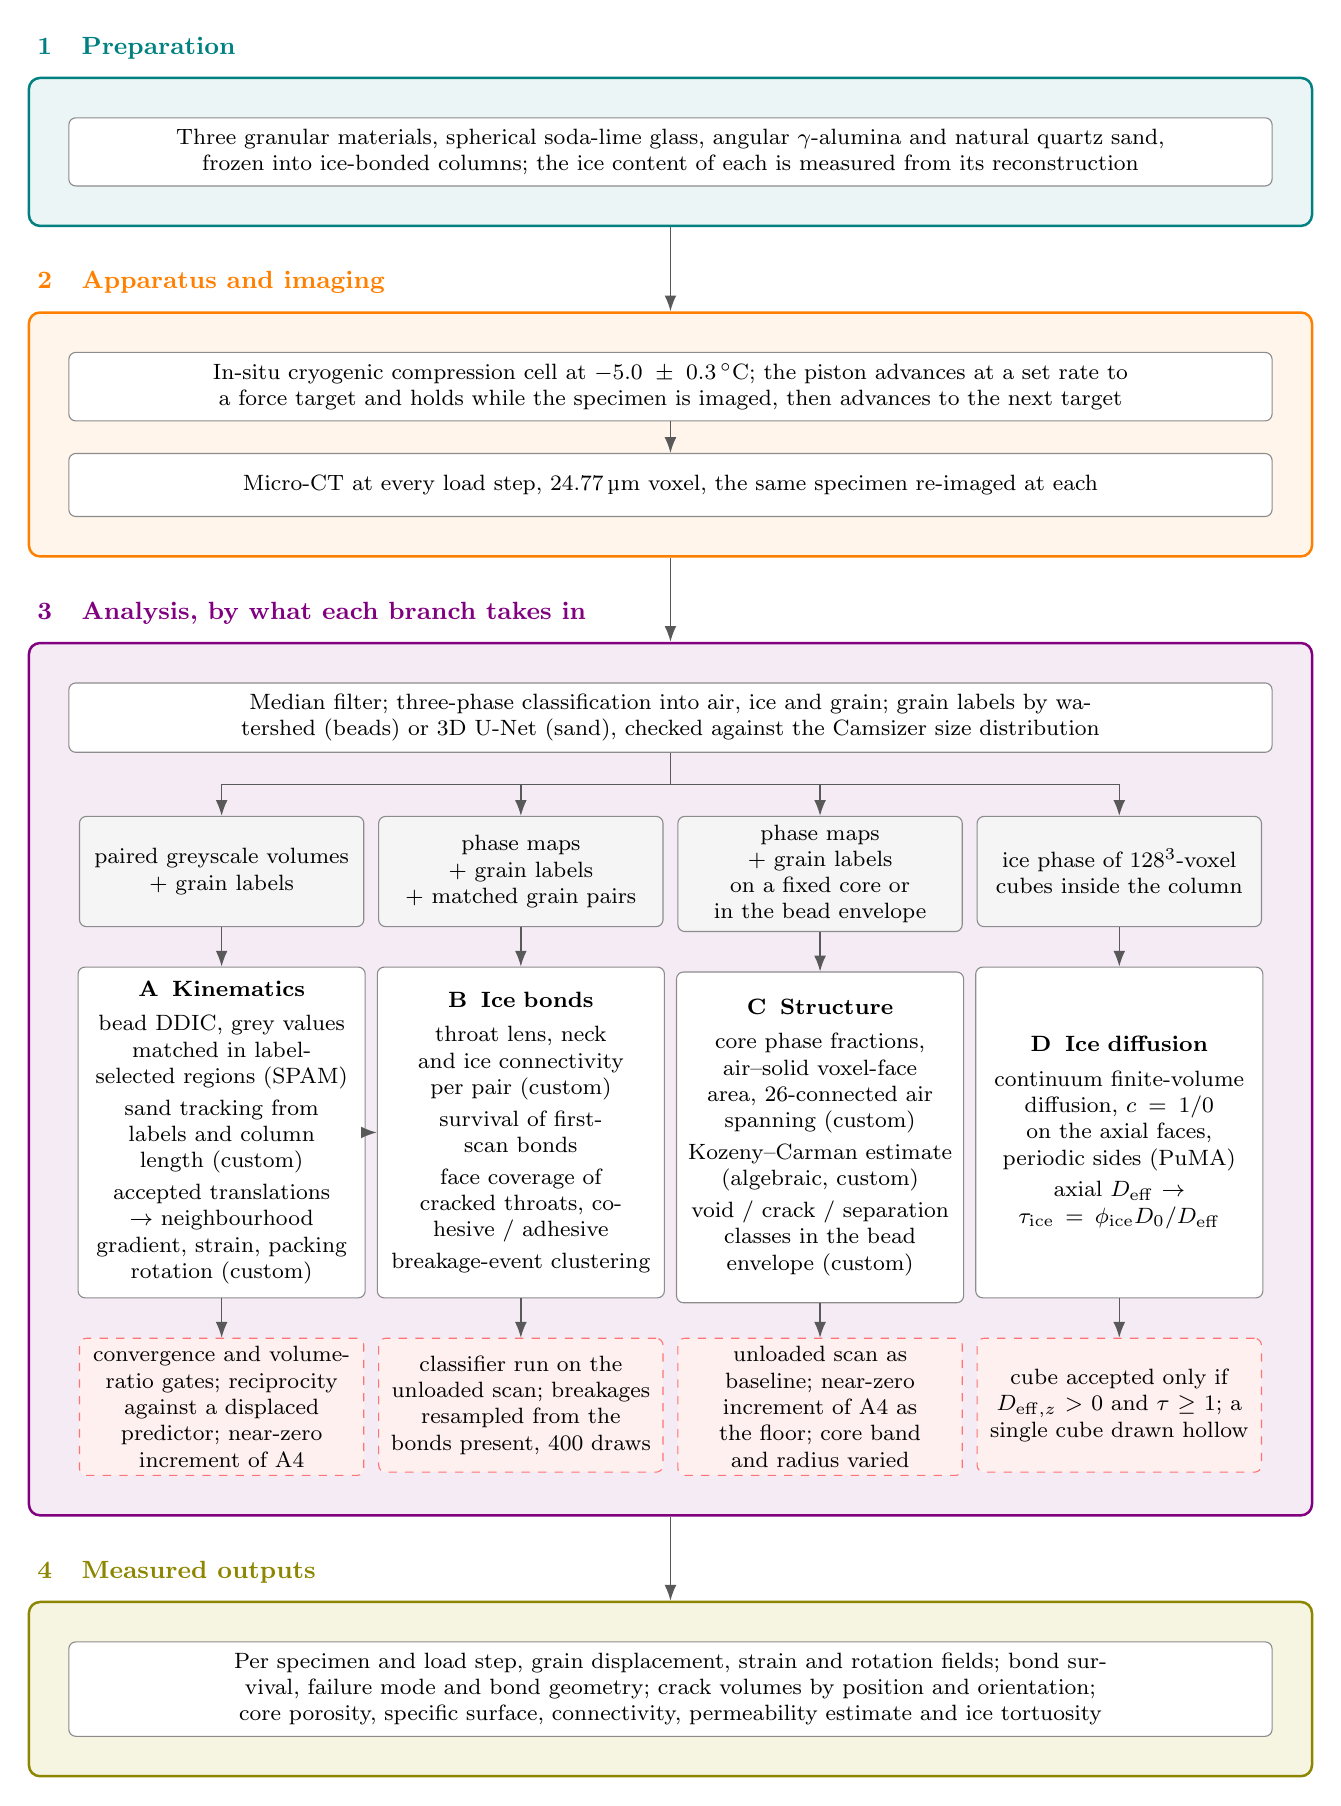
\begin{tikzpicture}[
    font=\footnotesize,
    stage/.style={rectangle, rounded corners=2.5pt, draw=black!45,
                  fill=white, align=center, inner sep=4pt,
                  text width=#1, minimum height=8mm},
    inp/.style={rectangle, rounded corners=2.5pt, draw=black!45,
                fill=black!4, align=center, inner sep=3pt,
                text width=#1, minimum height=14mm},
    ana/.style={rectangle, rounded corners=2.5pt, draw=black!45,
                fill=white, align=center, inner sep=3.5pt,
                text width=#1, minimum height=42mm},
    ctrl/.style={rectangle, rounded corners=2.5pt, draw=red!55, dashed,
                 fill=red!6, align=center, inner sep=3pt, text width=#1,
                 minimum height=17mm},
    grp/.style={rectangle, rounded corners=4pt, draw=#1, line width=0.9pt,
                fill=#1!8, inner sep=5mm},
    tag/.style={anchor=south west, font=\small\bfseries, text=#1},
    ar/.style={-{Latex[length=2mm]}, draw=black!65, line width=0.5pt},
  ]

  \def\W{150mm}
  \def\B{34mm}

  % ---- 1. preparation -------------------------------------------------------
  \node[stage=\W] (mat) at (0,0)
    {Three granular materials, spherical soda-lime glass, angular
     $\gamma$-alumina and natural quartz sand, frozen into ice-bonded columns;
     the ice content of each is measured from its reconstruction};

  % ---- 2. apparatus and acquisition ----------------------------------------
  \node[stage=\W, below=21mm of mat] (rig)
    {In-situ cryogenic compression cell at $-5.0\pm0.3\,^\circ$C; the piston
     advances at a set rate to a force target and holds while the specimen is
     imaged, then advances to the next target};
  \node[stage=\W, below=4mm of rig] (ct)
    {Micro-CT at every load step, \SI{24.77}{\micro\meter} voxel, the same
     specimen re-imaged at each};

  % ---- 3. analysis ----------------------------------------------------------
  \node[stage=\W, below=21mm of ct] (pre)
    {Median filter; three-phase classification into air, ice and grain;
     grain labels by watershed (beads) or 3D U-Net (sand), checked against
     the Camsizer size distribution};
  \node[inp=\B, below=8mm of pre, xshift=-57mm] (iA)
    {paired greyscale volumes\\+ grain labels};
  \node[inp=\B, below=8mm of pre, xshift=-19mm] (iB)
    {phase maps + grain labels\\+ matched grain pairs};
  \node[inp=\B, below=8mm of pre, xshift=19mm] (iC)
    {phase maps + grain labels\\on a fixed core or\\in the bead envelope};
  \node[inp=\B, below=8mm of pre, xshift=57mm] (iD)
    {ice phase of $128^3$-voxel\\cubes inside the column};

  \node[ana=\B, below=5mm of iA] (kin)
    {\textbf{A\enspace Kinematics}\\[3pt]
     bead DDIC, grey values matched in label-selected regions (SPAM)\\[2pt]
     sand tracking from labels and column length (custom)\\[2pt]
     accepted translations $\to$ neighbourhood gradient, strain, packing
     rotation (custom)};
  \node[ana=\B, below=5mm of iB] (bond)
    {\textbf{B\enspace Ice bonds}\\[3pt]
     throat lens, neck and ice connectivity per pair (custom)\\[2pt]
     survival of first-scan bonds\\[2pt]
     face coverage of cracked throats, cohesive / adhesive\\[2pt]
     breakage-event clustering};
  \node[ana=\B, below=5mm of iC] (str)
    {\textbf{C\enspace Structure}\\[3pt]
     core phase fractions, air--solid voxel-face area, 26-connected air
     spanning (custom)\\[2pt]
     Kozeny--Carman estimate (algebraic, custom)\\[2pt]
     void / crack / separation classes in the bead envelope (custom)};
  \node[ana=\B, below=5mm of iD] (tra)
    {\textbf{D\enspace Ice diffusion}\\[3pt]
     continuum finite-volume diffusion, $c=1/0$ on the axial faces,
     periodic sides (PuMA)\\[2pt]
     axial $D_\mathrm{eff}$ $\to$
     $\tau_\mathrm{ice}=\phi_\mathrm{ice}D_0/D_\mathrm{eff}$};

  \node[ctrl=\B, anchor=north] (cA) at ([yshift=-5mm]kin.south |- kin.south)
    {convergence and volume-ratio gates; reciprocity against a displaced
     predictor; near-zero increment of A4};
  \node[ctrl=\B, anchor=north] (cB) at ([yshift=-5mm]bond.south |- kin.south)
    {classifier run on the unloaded scan; breakages resampled from the
     bonds present, 400 draws};
  \node[ctrl=\B, anchor=north] (cC) at ([yshift=-5mm]str.south |- kin.south)
    {unloaded scan as baseline; near-zero increment of A4 as the floor;
     core band and radius varied};
  \node[ctrl=\B, anchor=north] (cD) at ([yshift=-5mm]tra.south |- kin.south)
    {cube accepted only if $D_{\mathrm{eff},z}>0$ and $\tau\ge1$;
     a single cube drawn hollow};

  % ---- 4. outputs -----------------------------------------------------------
  \coordinate (cmid) at (0,0 |- cA.south);
  \node[stage=\W, below=21mm of cmid] (res)
    {Per specimen and load step, grain displacement, strain and rotation
     fields; bond survival, failure mode and bond geometry; crack volumes by
     position and orientation; core porosity, specific surface, connectivity,
     permeability estimate and ice tortuosity};

  % ---- the four stage containers ------------------------------------------
  \begin{scope}[on background layer]
    \node[grp=teal,   fit=(mat)]                        (gA) {};
    \node[grp=orange, fit=(rig)(ct)]                    (gB) {};
    \node[grp=violet, fit=(pre)(iA)(iD)(cA)(cD)]        (gC) {};
    \node[grp=olive,  fit=(res)]                        (gD) {};
  \end{scope}
  \node[tag=teal]   at ([yshift=1mm]gA.north west) {1\quad Preparation};
  \node[tag=orange] at ([yshift=1mm]gB.north west) {2\quad Apparatus and imaging};
  \node[tag=violet] at ([yshift=1mm]gC.north west) {3\quad Analysis, by what each branch takes in};
  \node[tag=olive]  at ([yshift=1mm]gD.north west) {4\quad Measured outputs};

  % ---- flow -----------------------------------------------------------------
  \draw[ar] (gA.south) -- (gB.north);
  \draw[ar] (gB.south) -- (gC.north);
  \draw[ar] (gC.south) -- (gD.north);
  \draw[ar] (rig) -- (ct);
  \foreach \i/\n/\c in {iA/kin/cA, iB/bond/cB, iC/str/cC, iD/tra/cD}{
    \draw[ar] (pre.south) -- ++(0,-4mm) -| (\i.north);
    \draw[ar] (\i) -- (\n);
    \draw[ar] (\n) -- (\c);
  }
  % the bond branch also takes the matched pairs of the kinematics branch
  \draw[ar, dashed] (kin.east) -- (bond.west);
\end{tikzpicture}
}
    \caption{Analysis workflow.  Paired images with grain labels give the
      kinematics, the phase maps give the bond, structural and crack
      measures, and the ice phase of interior cubes gives the diffusion
      tortuosity.  Package operations are named, everything else is the
      authors' own code, and the Kozeny--Carman permeability is a
      geometry-based estimate.}
    \label{fig:pipeline}
  \end{figure}

  \subsection{Granular materials and specimen preparation}
  \label{sec:materials}
  Three granular materials were selected to investigate how particle morphology
  governs inter-particle ice-bond formation, bond failure modes, and grain-scale
  damage mechanisms under uniaxial compression, namely spherical soda-lime
  \emph{glass beads}, angular \emph{$\gamma$-alumina}
  ($\gamma$-Al$_2$O$_3$), and natural \emph{quartz sand}.
  The materials span a deliberate range from perfectly spherical and smooth to
  angular and rough, enabling a systematic comparison of how grain shape
  affects the ice-bond network geometry and the sequence of bond-breakage
  events observed in situ.
  The glass beads are from the same batch as the companion
  study~\cite{Khosrozadeh2026inverse}, where the supplier, particle density and
  size distribution are reported in full.  All five glass specimens use the
  coarse grade of nominal \SIrange{1700}{1800}{\micro\meter}, whose size
  distribution was measured by dynamic image analysis at
  $D_{50}=\SI{1722}{\micro\meter}$ (Section~\ref{sec:res_microstructure}).  The
  $\gamma$-alumina particles were supplied by Sasol~Germany~GmbH in two nominal
  sieve fractions of \SI{1000}{\micro\meter} and \SI{1800}{\micro\meter}.
  The particle-size distribution of the quartz sand was measured by dynamic
  image analysis (Camsizer~XT, Retsch Technology, Germany), and the results
  are presented in Section~\ref{sec:res_microstructure}.
  The glass beads were additionally tested in two surface-roughness
  conditions, smooth as-received and roughened, the latter denoted HR.  The HR
  beads were abraded in a mortar for about \SI{2}{\hour} with silicon carbide
  paste (grade F400) following Bunke et al.~\cite{BUNKE2024151016}, and their
  diameter was re-checked afterwards to confirm that sphericity was preserved.
  Confocal laser-scanning microscopy (Keyence VK-X160K, Japan) gives a mean
  areal roughness $S_a$ of $28.7 \pm \SI{4}{\nano\meter}$ for the HR beads
  against $17.7 \pm \SI{3}{\nano\meter}$ for the smooth ones.  That difference
  is three orders of magnitude below the \SI{24.77}{\micro\meter} voxel size,
  so it cannot be resolved in the reconstructions and enters this study only
  through the grain-scale contact and damage metrics of
  \S\ref{sec:analysis}.

  Specimens were prepared as \emph{ice-bonded} granular packings following
  \cite{Khosrozadeh2026inverse} at two nominal saturation levels, partially
  saturated ($w_\mathrm{nom} \approx \SI{75}{\percent}$) and fully saturated
  ($w_\mathrm{nom} \approx \SI{100}{\percent}$)~\cite{Chan2022}.
  Because the as-prepared water content could not be measured precisely during
  preparation, the \emph{ice content of each specimen is quantified directly from
  the reconstructed images} as the volume fraction of the segmented ice phase
  (Section~\ref{sec:segmentation}), and this measured value, rather than the
  nominal preparation one, is used as the controlling variable throughout.

  The measured ice volume fraction $\phi_\mathrm{ice}$ of each specimen is
  reported in Table~\ref{tab:matrix} (Section~\ref{sec:res_microstructure}),
  alongside its dimensions, grain size and the other phase fractions.

  \subsection{In-situ compression and freezing apparatus}
  \label{sec:apparatus}
  A custom apparatus was built to apply uniaxial compression and maintain a
  controlled sub-zero temperature \emph{in situ}, so that the same specimen could
  be imaged repeatedly under increasing load without being removed from the
  micro-CT scanner (Figure~\ref{fig:apparatus}).
  \begin{figure}[htbp]
    \centering
    \begin{subfigure}[b]{\linewidth}
      \centering
      \includegraphics[width=\linewidth]{figures/apparatus_cad.png}
      \caption{assembly, with the compression device outlined}
      \label{fig:apparatus_cad}
    \end{subfigure}

    \vspace{10pt}
    \begin{subfigure}[b]{\linewidth}
      \centering
      \includegraphics[width=\linewidth]{figures/apparatus_cell.png}
      \caption{the compression device in section}
      \label{fig:apparatus_cell}
    \end{subfigure}
    \caption{The in-situ cryogenic compression apparatus.}
    \label{fig:apparatus}
  \end{figure}

  \begin{figure}[htbp]\ContinuedFloat
    \centering
    \begin{subfigure}[b]{\linewidth}
      \centering
      \includegraphics[width=\linewidth]{figures/apparatus_photo.png}
      \caption{mounted on the stage, with the specimen and the field of view
        inset}
      \label{fig:apparatus_photo}
    \end{subfigure}
    \caption{(continued)}
  \end{figure}

  Uniaxial compression is applied by a NEMA-17 stepper motor
  (17HS19-2004S1, \num{200} full steps per revolution, \SI{1.8}{\degree}) driving
  a \SI{2}{\milli\meter}-pitch lead screw, which advances a loading piston upward
  against the specimen. The motor is driven by a TB6600 driver at
  \num{32}$\times$ microstepping (\num{3200} microsteps per millimetre, a nominal
  displacement resolution of $\approx$\,\SI{0.31}{\micro\meter}) and commanded by an
  Arduino Due. The axial force is measured by an in-line \SI{500}{\newton}
  compression load cell (ME-Messsysteme KM10a), whose bridge signal is conditioned
  by a GSV-14L amplifier and digitised by a 16-bit ADS1115 analogue-to-digital
  converter read by the Arduino. The maximum piston travel is \SI{10}{\milli\meter}.
  Prior to the experiments, the load cell was calibrated against known deadweights
  over the full range 0--\SI{410}{\newton}, and a linear fit to the ten
  calibration points yielded $F\,(\si{\newton}) = 0.2840\,V_\mathrm{mV} - 375.42$
  ($R^2 = 0.9994$), which was applied to all recorded bridge voltages.
  The specimen is enclosed in a thin-walled poly(methyl methacrylate, PMMA)
  cylinder (\SI{15}{\milli\meter} inner diameter, \SI{0.5}{\milli\meter}
  wall thickness), chosen for its low X-ray attenuation to minimise imaging
  artefacts. An aluminium insert (\SI{13}{\milli\meter} inner diameter) acts
  as the loading piston in direct contact with the specimen.  Its high thermal
  conductivity also ensures a uniform radial temperature distribution, which
  compensates for the absence of air circulation within the sealed device.

  The specimen is held at a constant sub-zero temperature by two Peltier
  (thermoelectric) elements (TRU~COMPONENTS TEC1-127080, \SI{15.4}{\volt},
  \SI{8.5}{\ampere}, \SI{72}{\watt}, $40\times40\times3.3$\,\si{\milli\meter}),
  whose hot sides are dissipated by a closed-loop all-in-one liquid cooler
  (Xilence LQ360, pump and radiator fans). The Peltier elements are driven by a
  proportional thermoelectric controller (Quick-Ohm QC-PC-C01C,
  input \SIrange{10}{24}{\volt}\,DC, maximum output \SI{10}{\ampere},
  NTC \SI{10}{\kilo\ohm} sensor, $\beta = \SI{3977}{\kelvin}$), with the
  target temperature set via a \SI{10}{\kilo\ohm} potentiometer.  The actual
  and target temperatures are displayed on a Quick-Ohm QC-PC-D-100 unit.
  All experiments used a controller set point of \SI{-15}{\celsius}.  Because
  the micro-CT scanner environment is maintained at approximately
  \SI{20}{\celsius}, the thermal equilibrium between the Peltier cooling and
  the ambient heat load stabilised the specimen-chamber temperature at
  $-5.0 \pm 0.3$\,\si{\celsius}, as confirmed by the on-device display.
  Prior to each test, the aluminium holder, PMMA cylinder, cap and load cell
  were pre-chilled in a \SI{-18}{\celsius} freezer and dry ice was placed on
  the piston cap to accelerate equilibration.  No scan was started until the
  steady-state temperature of \SI{-5}{\celsius} had been reached
  (approximately \SI{15}{\minute}).

  Tests were run under displacement control to a force target.  After taring
  the load cell, the piston advanced at a constant rate, between
  \SI{0.010}{} and \SI{0.60}{\milli\meter\per\second} depending on the
  specimen (Table~\ref{tab:matrix}), which on a \SI{20}{}--\SI{27}{\milli\meter}
  column is a nominal strain rate of $4\times10^{-4}$ to
  $3\times10^{-2}\,\si{\per\second}$, until the measured axial force reached a
  prescribed target, whereupon motion stopped and the position was held while
  a full tomographic scan was acquired. The target force was then increased
  and the sequence repeated, producing a series of load steps imaged at
  successively higher load. Throughout each test, force and piston displacement
  were logged continuously at \SI{10}{\hertz}, giving a force--displacement
  record for every specimen.  The load cell was recalibrated after these tests
  (\ref{app:calibration}), and the in-situ traces acquired before that
  calibration are not used quantitatively here.  The load levels quoted are
  therefore those of the companion compression tests against which the targets
  were set.
  To establish appropriate force targets, a preliminary quasi-static
  compression test without CT scanning was first performed for each material to
  identify the failure load, and the in-situ tests then targeted a fixed
  fraction of it, about $60\%$ at the intermediate step and the failure load
  itself at the last.  Three scans per specimen were planned, an unloaded one,
  an intermediate one and one near failure, although practical constraints
  meant this was not always achieved.

  \subsection{Micro-CT acquisition}
  \label{sec:ct}
  Tomographic imaging was performed at the RPTU Kaiserslautern MVT CT laboratory
  on a Werth Messtechnik TomoScope L 300, equipped with a
  \SI{240}{\kilo\volt}/\SI{80}{\watt} microfocus X-ray tube (F240T80, minimum
  focal-spot size \SI{3.5}{\micro\meter}) and a $4000\times4000$-pixel PerkinElmer
  PE4000 flat-panel detector (\SI{100}{\micro\meter} pixel pitch,
  $400\times400$\,\si{\milli\meter}). All scans were acquired at
  \SI{150}{\kilo\volt} and \SI{300}{\micro\ampere} with no beam filter and
  \SI{267}{\milli\second} integration time per projection (no frame averaging).
  Glass and $\gamma$-alumina scans comprised \num{1000} projections over
  \SI{360}{\degree} and took about \SI{30}{\minute} each, while the sand scans
  used \num{900} projections and took about \SI{31}{\minute}. The source-to-object and source-to-detector
  distances were \SI{270}{\milli\meter} and \SI{1072}{\milli\meter} (geometric
  magnification $\approx 3.97$), giving a reconstructed voxel size of
  \SI{24.77}{\micro\meter} (volume $\approx 996\times1179\times1179$ voxels),
  identical for all three materials.
  The source-to-object distance of \SI{270}{\milli\meter} was set by the
  safety clearance the present cell requires from the X-ray tube, and it is
  what fixes the voxel size (\S\ref{sec:disc_sandres}).

  \subsection{Image processing and segmentation}
  \label{sec:segmentation}

  Each reconstructed greyscale volume was processed in three stages, namely
  noise filtering, three-phase classification into interior air void, ice and
  grain, and grain instance labelling.  The first two were common to all
  materials, and the third differed because the grain morphologies make
  classical instance segmentation impractical for sand.

  \subsubsection{Specimen mask and phase classification}
  A $3\times3\times3$ voxel 3D median filter was applied to each volume to
  suppress detector noise while preserving grain boundaries.  A specimen mask
  was then derived slice by slice.  Each axial cross-section was thresholded
  to separate solid material from the surrounding air, the largest connected
  component was retained, and any interior holes were filled, which produces a
  binary mask of the specimen interior for all subsequent steps.

  Within the specimen mask, the greyscale histogram shows three distinct peaks
  corresponding to interior air voids (lowest intensity), ice (intermediate),
  and grains (highest), reflecting the density contrast among the three phases.
  For glass and $\gamma$-alumina specimens, fixed intensity thresholds at the two
  inter-peak valleys were identified from the histogram of a representative
  axial slice and applied uniformly throughout the volume.  For sand specimens,
  a pronounced axial intensity drift (arising from beam-hardening and
  cone-beam geometry) caused the inter-peak positions to shift along the
  $z$-axis, so thresholds were determined independently for each slice by
  three-class Otsu optimisation and smoothed along $z$ before application.
  This per-slice adaptive approach is essential for the full sand stack and
  constitutes the principal source of residual ice/sand misclassification in
  the classical segmentation, and it is one motivation for the deep-learning
  approach described below.  Fig.~\ref{fig:seg_hist} shows the histograms and
  the two thresholds taken from them.

  \begin{figure}[htbp]
    \centering
    \includegraphics[width=\linewidth]{figures/seg_histogram.pdf}
    \caption{Specimen greyscale histograms for $\gamma$-alumina (left) and glass (right), with the three-class Otsu thresholds dashed.}
    \label{fig:seg_hist}
  \end{figure}

  \subsubsection{Grain segmentation and its validation}
  \label{sec:sanddl}
  For glass and $\gamma$-alumina, where grains are near-spherical (glass) or
  blocky ($\gamma$-alumina), large (1000--1800\,\si{\micro\meter}), and reasonably well
  separated, individual grain labels were obtained by a marker-controlled
  watershed implemented in ORS Dragonfly (version~2025.1, Object Research
  Systems, Montreal, Canada).  First, the Euclidean distance transform (EDT) of the grain-phase binary
  mask was computed, and an H-maxima filter then suppressed all maxima of height
  less than $h = 1.0$ voxels, retaining one seed marker per grain interior.
  The watershed algorithm was subsequently applied to the inverted EDT,
  growing each seed to its basin boundary.  Connected objects below a minimum volume of
  \num{20}\,voxels were discarded as noise.
  Figure~\ref{fig:seg} illustrates the complete workflow for both bead
  materials, from the greyscale CT slice through the three-phase segmentation
  with the detected specimen contour to the resulting individual grain labels.

  \begin{figure}[htbp]
    \centering
    \includegraphics[width=\linewidth]{figures/seg_glass_alumina.pdf}
    \caption{Segmentation workflow for the bead materials, with $\gamma$-alumina (top) and glass (bottom).}
    \label{fig:seg}
  \end{figure}

  Classical watershed severely over-segments angular, polydisperse sand grains
  because extended planar grain--grain contacts prevent the EDT from finding
  unique interior maxima.  Sand grains were therefore segmented using the
  \emph{border--core} label representation introduced by
  Gotkowski~et~al.~\cite{Gotkowski2024}, in which a 3D U-Net is trained to
  classify each voxel as background (ice or air), grain \emph{core} (eroded
  grain interior), or grain \emph{border} (contact shell).  Instance labels are recovered by
  connected-components labelling of the core prediction followed by a constrained
  watershed that is suppressed by the border channel, preventing propagation across
  contact planes.

  The network was implemented as a compact 3D U-Net encoder--decoder~\cite{Cicek2016}
  with group normalisation, trained on 96\textsuperscript{3}-voxel patches using AdamW
  optimisation and a combined cross-entropy and soft-Dice loss with an upweighted
  border class.  No pretrained weights were used, and the model was trained from scratch on
  synthetic volumes generated in-house.  Grain shapes were drawn from the
  Sand~Atlas library~\cite{Vego2025} (Hamburg, Ottawa, and Hostun sand datasets),
  packed into dense touching configurations, and rendered at the scan grayscale
  statistics (24.77\,\si{\micro\meter} voxel size, matched noise, Gaussian PSF).
  A first model variant (v1) used uniform sand intensity throughout, while a
  second variant (v2) also injected a thin ice-intensity dip at grain--grain
  contacts to simulate the ice-neck grey signature present in the frozen
  specimens.  To select the final model, a five-way comparison was conducted on the
  initial scan of each specimen series against the adaptive watershed, the v1
  model, ParticleSeg3D~\cite{Gotkowski2024} applied zero-shot with released
  weights, and Cellpose-SAM~4.1.1~\cite{Pachitariu2025} applied zero-shot.  The v2 model
  gave the lowest grain-size error in two of the three specimens and lay
  within two points of the watershed in the third, while both external models
  merged the packing into a few hundred labels, and v2 was therefore selected;
  the comparison is reported in Section~\ref{sec:res_microstructure}.
  Full-volume inference was applied to all seven sand scans at the native
  $996\times1179\times1179$ voxel resolution.

  Fig.~\ref{fig:grainplate} shows the segmented particles of all three
  materials at the first load step, rendered from the label volumes at full
  resolution.  Voxels on a face shared by two labels are cleared before
  meshing, so that touching particles do not weld into one surface; this trims
  about one voxel from each rim and is a drawing device only.  The bead panels
  contain every bead in the specimen, 369 in G1 and 344 in A4, while the sand
  panel is a \SI{1.4}{\milli\meter} slab holding \num{56475} of that
  specimen's \num{287276} grains, which cannot be meshed whole.  The three are
  placed together for the contrast in particle shape between the
  near-spherical glass, the faceted $\gamma$-alumina and the angular sand, the
  property that distinguishes the materials and that
  \S\ref{sec:disc_morphology} returns to.

\begin{figure}[htbp]
    \centering
    \begin{subfigure}[b]{0.31\linewidth}
      \includegraphics[width=\linewidth]{figures/grains_glass.png}
      \caption{glass, G1}
      \label{fig:grains_glass}
    \end{subfigure}\hfill
    \begin{subfigure}[b]{0.31\linewidth}
      \includegraphics[width=\linewidth]{figures/grains_alumina.png}
      \caption{$\gamma$-alumina, A4}
      \label{fig:grains_alumina}
    \end{subfigure}\hfill
    \begin{subfigure}[b]{0.31\linewidth}
      \includegraphics[width=\linewidth]{figures/grains_sand.png}
      \caption{quartz sand, S2}
      \label{fig:grains_sand}
    \end{subfigure}
    \caption{Segmented particles of the three materials at the first load step, one colour per particle.}
    \label{fig:grainplate}
  \end{figure}

  For each material, the grain-size distribution obtained from the initial
  (unloaded) scan was compared against a reference to validate the instance
  segmentation, namely Camsizer~XT measurements of the same powder for the glass beads
  and quartz sand, and the supplier nominal grades for the $\gamma$-alumina
  beads. The volumetric ice content,
  \begin{equation}
    \phi_\mathrm{ice} = \frac{V_\mathrm{ice}}{V_\mathrm{interior}},
  \end{equation}
  where $V_\mathrm{ice}$ is the volume of ice-labelled voxels and
  $V_\mathrm{interior} = V_\mathrm{grain}+V_\mathrm{ice}+V_\mathrm{air}$ the
  total specimen-interior volume, is used as the measured ice fraction
  throughout this study. The degree of ice saturation,
  \begin{equation}
    S = \frac{V_\mathrm{ice}}{V_\mathrm{ice}+V_\mathrm{air}}
      = \frac{\phi_\mathrm{ice}}{1-\rho},
  \end{equation}
  where $\rho$ is the particle packing fraction, quantifies the fraction of the
  inter-particle void space occupied by ice, and it is the measured counterpart
  of the nominal saturation level targeted during specimen preparation.

  \subsection{Quantitative analysis}
  \label{sec:analysis}

  Grain-scale kinematics, the ice-bond network, and macrostructural transport
  properties were extracted from the labelled volumes using two open-source
  toolkits, SPAM (Software for Practical Analysis of
  Materials~\cite{Stamati2020}) for grain tracking and contact/bond analysis,
  and PuMA (Porous Microstructure Analysis~\cite{Ferguson2021}) for structural
  and transport properties.

  \subsubsection{Grain kinematics and strain}
  \label{sec:ddic}
  \label{sec:sandtrack}
  \label{sec:sandstrain}
  Per-grain displacement between successive load steps was obtained by discrete
  digital volume correlation (DDIC) using SPAM~0.9~\cite{Stamati2020}.  The
  inputs are the two greyscale reconstructions and the grain labels of the
  first of them; the labels only select the region correlated, and what is
  matched is grey value.  For grain $i$ occupying the voxels $\Omega_i$ of
  scan $A$, the solver finds the transformation $\Phi$ that minimises the
  grey mismatch
  \begin{equation}
    \mathcal{E}(\Phi) = \tfrac12 \sum_{\mathbf{x}\in\Omega_i}
      \bigl[\, I_A(\mathbf{x}) - I_B\bigl(\mathbf{x}_c + \mathbf{t}
      + \mathbf{F}_i(\mathbf{x}-\mathbf{x}_c)\bigr) \bigr]^2 ,
    \label{eq:ddic}
  \end{equation}
  where $I_A$ and $I_B$ are the two images, $\mathbf{x}_c$ the grain centroid,
  $\mathbf{t}$ the translation and $\mathbf{F}_i$ the affine part of $\Phi$,
  by the incremental Gauss--Newton (Lucas--Kanade) iteration of
  Ref.~\cite{Stamati2020}, with the updated-gradient option, a two-level
  coarse-to-fine start and a per-grain seed.  Each grain is correlated over a
  subvolume extending 15~voxels (\SI{370}{\micro\meter}) beyond its segmented
  bounding box, with the label dilated by two voxels to admit the grain
  boundary, since the grey gradient at the boundary is the texture a smooth
  bead offers.  A full affine $\Phi$ is fitted per grain, but only its
  translation is used,
  since a smooth sphere carries no internal texture from which its own spin
  could be recovered.  The rotation quoted below is the rotation of the
  \emph{local packing}, taken from the polar decomposition of the deformation
  gradient fitted over each grain's neighbours (Eq.~\eqref{eq:gradu}) after
  the rigid motion of the whole column has been removed; it says how far the
  neighbourhood of a grain has turned, not how far the grain has spun.

  Three settings were necessary rather than conventional.  The iteration cap
  was raised to 300, because at its default near-misses terminated with the
  incremental transformation norm $\|\Delta\Phi\|$ still at $0.016$ against a
  threshold of $0.001$, which took one specimen from 68 to 219 converged grains
  of 483.  A two-level multiscale pass was used because grains translate by of
  order one radius per load step and would otherwise begin outside their own
  convergence basin.  The first guess was geometric, its axial stretch and
  translation taken from the grain centroid cloud and its lateral stretch from
  the RMS radius of the centroids rather than from the specimen mask, which is
  unreliable where the outer boundary is partly ice.

  Reconstructed grey scales differ between scans by up to a factor of three to
  six, and the solver minimises a sum of squared grey-value differences, so a
  uniformly brighter scan begins every correlation with a residual that no
  iteration can remove.  Where the gain was material, a two-landmark linear map
  (pore, grain) was applied to a \emph{copy} of the second scan; the originals
  were never modified.  Volumes of differing raw dimensions were zero-padded at
  the high-index end, so every reported coordinate remains a raw-frame
  coordinate.

  The label image selects what is correlated, so any label admitted by the
  segmentation enters the displacement field as though it were a grain.  Labels
  failing the shape gate of \S\ref{sec:shapegate}, which are fragments of
  fractured grains and, in the $\gamma$-alumina specimens, portions of the
  punch, the support and the confining wall, were therefore excluded before any
  kinematic quantity was computed.  Grains were retained
  as usable at return\,status\,$\geq 1$ and counted as converged at
  return\,status\,$\geq 2$.  DDIC was applied to all nine bead specimens
  (G1--G5, A1--A4).  A blind grey-value correlation is not feasible for the
  quartz sand (S1--S3), where the fine, near-periodic packing yields incoherent
  displacement fields, with residuals of several grain diameters after
  rigid-body removal.  The sand grains can nevertheless be followed
  individually by a different route, described in \S\ref{sec:sandtrack}.

  A continuum displacement field was also computed for the sand by local
  digital volume correlation (LDIC) on $2\times$-downsampled volumes,
  $41^3$-voxel windows of \SI{2.0}{\milli\meter} edge on a
  \SI{0.99}{\milli\meter} node grid.  It is used only as the coarse predictor
  that the grain tracking below starts from and refines, since on its own it
  converges on too few nodes at the larger load steps to give a strain field.


  The blind correlation described above fails in quartz sand, and the reason is geometric rather than photometric. The packing is near-periodic at the grain
  scale, so a grain one position away correlates almost as well as the right
  one and an exhaustive search has no basis on which to choose.  A local search
  does not have that problem, and two things make the search local.  Deep
  learning supplies grain labels in \emph{both} scans of a pair
  (\S\ref{sec:sanddl}), so both centroid sets are known without any
  correlation, and the column length is measured in each scan from the axial
  texture profile,
  without correlation of any kind, so the affine part of the motion is known in
  advance.  A grain at height $p_z$ in scan~$A$ is predicted at $p_z F_{zz}$ in
  scan~$B$, with
  \begin{equation}
    F_{zz} \;=\; \frac{L_B}{L_A},
    \label{eq:fzz}
  \end{equation}
  where $F_{zz}$ is the axial stretch and $L_A$ and $L_B$ are the column
  lengths measured in the two scans.  Each grain is then
  matched to the nearest scan-$B$ centroid, and the predictor is rebuilt from
  the accepted matches themselves, as the median displacement of the twelve
  nearest accepted grains, and the matching repeated, which sharpens the
  prediction from the $\SI{0.99}{\milli\meter}$ node spacing of a continuum
  field to the spacing of the grains.

  A match is accepted only if it is closer than half the mean grain spacing, if
  the runner-up is at least $1.6\times$ further away, and if the two grains have
  volumes within a factor $0.6$--$1.6$, a grain being rigid.  None of those
  three tests can establish that a match is \emph{correct}, since each is
  satisfied by construction or by any pair drawn from the same size
  distribution.  Correctness is therefore established by \textbf{reciprocity},
  in that scan~$B$ is tracked back to scan~$A$ as an independent problem and only
  pairs for which grain~$i$ chooses~$j$ \emph{and} $j$ independently chooses
  $i$ are retained.  Against a deliberate null, in which the forward prediction
  is displaced by half a grain spacing so that every match is wrong by
  construction, ${\approx}9400$ matches are still accepted on residual and
  volume ratio and yet reciprocity for every one of them is \emph{zero}.
  Reciprocity therefore rejects the error that a nearest-centroid match makes
  most readily.  It cannot reject a match that is wrong by a whole grain
  spacing in a near-periodic packing, since such a match is reciprocal by
  construction, and at the largest load steps the number of accepted matches
  was found not to depend on the seed offset; the fields of
  \S\ref{sec:res_sandkin} are therefore read for their pattern and their
  magnitude rather than grain by grain, and the sand strain is not carried
  into any bond or crack statistic.

  Strain in sand is computed from the tracked grains rather than from the
  continuum field, because the continuum correlation converges on only
  $1.6$--$1.7\%$ of nodes at the largest load steps and returns a volumetric
  strain of $-0.47$ against a specimen whose measured volume changes by $0.2\%$.
  The estimator is the one used for the beads, so that the three materials
  are compared on one definition, a least-squares fit of the displacement
  gradient over the nearest neighbours, 12 for the beads and 16 for the finer
  sand,
  \begin{equation}
    \min_{\mathbf{G},\,\mathbf{c}} \sum_{j\in\mathcal{N}(i)}
      \bigl\| \mathbf{u}_j - \mathbf{u}_i
              - \mathbf{G}\,(\mathbf{x}_j - \mathbf{x}_i) - \mathbf{c} \bigr\|^2 ,
    \label{eq:gradu}
  \end{equation}
  where $\mathbf{x}_i$ and $\mathbf{u}_i$ are the reference position and the
  displacement of grain $i$, $\mathcal{N}(i)$ is the set of its nearest
  neighbours, $\mathbf{G}$ is the fitted displacement gradient and $\mathbf{c}$
  a constant offset.  The fitted gradient is decomposed as Green--Lagrange
  through the deformation gradient $\mathbf{F} = \mathbf{G} + \mathbf{I}$,
  \begin{equation}
    \mathbf{E} \;=\; \tfrac{1}{2}\!\left(\mathbf{F}^{\mathsf{T}}\mathbf{F}
                     - \mathbf{I}\right),
    \label{eq:greenlagrange}
  \end{equation}
  in which $\mathbf{E}$ is the Green--Lagrange strain tensor and $\mathbf{I}$
  the identity tensor.  The equivalent strain quoted throughout is
  \begin{equation}
    E_\mathrm{eq} = \sqrt{\tfrac{2}{3}\,\mathbf{E}^{\mathrm{d}}\!:\!\mathbf{E}^{\mathrm{d}}},
    \qquad
    \mathbf{E}^{\mathrm{d}} = \mathbf{E} - \tfrac13\,\mathrm{tr}(\mathbf{E})\,\mathbf{I},
    \label{eq:eqstrain}
  \end{equation}
  an unsigned measure of distortion.  The reference configuration is the
  unloaded scan.  Fields labelled $1\!\to\!N$ are not sums of increments,
  since finite increments with differing rotations do not add.  The per-grain
  translations are chained through the tracking, so that the displacement of
  a grain from scan~1 to scan~$N$ is known at its scan-1 position, and
  $\mathbf{G}$, $\mathbf{E}$ and the rotation are re-fitted from that
  composed field.  These are strains of the packing inferred from the motion
  of grain centres over a neighbourhood of a few grains, not strains inside
  any grain, and the rotation of Eq.~\eqref{eq:gradu} is likewise the turning
  of that neighbourhood.  The 12-neighbour stencil spans about three bead
  diameters, which is the resolution of the field; the node spacing is one
  grain and is not a resolution.
  The intercept $\mathbf{c}$ in Eq.~\eqref{eq:gradu} is not cosmetic, because without
  it, a one-sided neighbourhood, which is what every neighbourhood at a free
  surface is, returns a spurious gradient, and a null control on pure noise with
  no radial structure reproduced a perimeter-to-interior strain ratio of $1.31$
  where the correct answer is unity.  The finite measure of
  Eq.~\eqref{eq:greenlagrange} is required because the infinitesimal measure is
  not frame-indifferent at the rotations these packings develop, and would
  report a spurious strain for a grain that has only rotated.

  One axial convention is used throughout the paper.  The punch acts on the
  low-$z$ end of every reconstruction, so that $z$ increases from the punch
  towards the support, and every height axis and every render is drawn in that
  same sense, with the punch at the top of the panel and the support at the
  bottom.  Heights given as a fraction of the column are measured from the
  punch face.  The convention is fixed by the reconstructions themselves,
  because the punch-side end carries the raised grey level of the shorter
  surrounding cylinder, and it is the end at which the axial displacement
  gradient is steepest in every specimen while the support-side quarter moves
  as a rigid body.

  All displacements are referenced to the support end by fitting a rigid
  transform, a rotation and a translation by the Kabsch construction, to the
  grains in the support-side quarter of the column and subtracting it
  everywhere.  A constant offset is not sufficient, because the stage rotates as well as
  translates between scans, and on the unloaded control pair this amounts to a
  $0.73^\circ$ tilt, which would otherwise be reported as a
  $\SI{208}{\micro\meter}$ displacement gradient along the column.


  \subsubsection{Detection of localised damage and the grain shape gate}
  \label{sec:crackdetect}
  \label{sec:shapegate}
  Air inside a bead packing is classed by where it sits and how wide it is.
  The region measured is the same construction on every scan of a specimen,
  the \emph{bead envelope}, which is the per-slice closing of the bead labels
  by a disc of $1.25$ bead radii with its holes filled, dilated by four
  voxels to keep the ice skin on the outermost beads, and cut one bead
  diameter clear of each platen.  A per-scan specimen mask was tried first
  and abandoned, because under load such a mask steps out to the tube bore
  and takes in the scalloped air between the outer beads, which then counts
  as crack; on A4, whose first increment moved the beads by
  \SI{0.04}{\milli\meter} and left the ice volume unchanged, that mask
  reported \SI{300}{\milli\meter\cubed} of crack.  Inside the envelope every
  air voxel of the phase map is a \emph{gap}, and gaps are classed as
  \emph{void} where they form isolated bodies below \SI{2}{\milli\meter\cubed},
  as \emph{crack} where they belong to a larger body and lie within
  \SI{0.125}{\milli\meter} of solid, so an opening up to \SI{0.25}{\milli\meter}
  wide, and as \emph{separation} where the opening is wider.  Crack within a
  20-voxel (\SI{0.5}{\milli\meter}) skin of the envelope is \emph{surface}
  crack and the rest \emph{body} crack.  Bodies below 100 voxels are specks
  of the phase map and enter no class.  The envelope admits the same
  boundary concavities on every scan, so the unloaded scan carries a baseline,
  zero in the glass and \SIrange{40}{70}{\milli\meter\cubed} in the
  $\gamma$-alumina from its pre-existing pores, and the damage is the change
  from it.  The floor of that change is set by A4's first increment, which
  imposed a shortening of $0.01$ and returned $+43$ and $+19$
  \si{\milli\meter\cubed} of surface and body crack, so changes of that size
  are not read as damage.

  Whether damage in a specimen is localised onto a surface, or distributed
  through the volume, is a question that any single criterion can answer
  affirmatively by accident.  A plane fitted to any cloud of points returns an
  angle, and a clustering algorithm at a fixed neighbourhood radius returns
  clusters at some radius for any point set.  Five independent criteria were therefore
  applied to the sand specimens, each with a control drawn from the unloaded
  scan pair of the same material, and a result was accepted only where it beat
  that control.
  \begin{enumerate}\itemsep2pt
    \item \textbf{Bond separation.}  Pairs of tracked grains bonded in the first
      scan, meaning centres closer than $1.25\,(r_i + r_j)$, classified as broken
      where the centre-to-centre distance grew beyond a threshold set at the
      99th percentile of the unloaded pair.  Centre-to-centre rather than
      surface-to-surface, because the measured gap between grain surfaces
      \emph{increases} at every load step while the column is being compacted,
      which is segmentation drift and not separation.
    \item \textbf{New void.}  Air inside the specimen mask, thresholded on the
      first scan's grey scale and held fixed.
    \item \textbf{Connected loose region.}  The largest connected body of
      locally low solid fraction, swept over cut level.
    \item \textbf{Plane through the loose voxels.}  PCA and RANSAC fits, with
      the inlier fraction as the test of planarity.
    \item \textbf{Specimen outline.}  The height at which the specimen radius
      steps, followed azimuth by azimuth.
  \end{enumerate}
  Where a clustering scale had to be chosen, it was swept rather than fixed, and
  the resulting $p$-values corrected across the sweep with the
  Benjamini--Hochberg procedure, as for the bead specimens
  (\S\ref{sec:res_planar}).  Null distributions were built by resampling
  \emph{intact} bonds stratified by height, because breakage and measurement
  error both concentrate towards one end of the column and an unstratified null
  rewards either.

  Not every label returned by the segmentation is a grain, because fractured
  $\gamma$-alumina beads yield crescent-shaped fragments and the reconstruction
  also labels parts of the punch, the support and the confining wall.  A label
  was therefore admitted as a grain only if its \emph{fill}, the ratio of label
  volume to the volume of its own least-squares fitted sphere, was at least
  $0.85$, its \emph{roughness}, the RMS radial deviation from the fitted radius
  normalised by that radius, was at most $0.12$, and its fitted radius lay
  within $\pm25\%$ of the specimen median.  Fill is the criterion that
  discriminates a fractured bead, because a crescent retains a plausible radius
  and a plausible inertia ratio but cannot fill the sphere it fits, and the same
  gate is applied to the bond census and to the kinematic analysis so that both
  describe one population of objects.

  \subsubsection{Ice bonds, their failure and its spatial organisation}
  \label{sec:bonds}
  \label{sec:failuremode}
  \label{sec:planar}
  Two grain labels were declared \emph{in contact} if the binary dilation of
  one grain's mask by one voxel intersected the other grain's mask.  The set
  of all contact pairs constitutes the contact network for that scan, and the
  coordination number $z$ of each grain is the count of its contact partners.

  A bond is identified with the \emph{throat} between a neighbouring pair.  For
  grains $A$ and $B$ with surface distances $d_A$ and $d_B$ and free gap $g$,
  free space along the shortest path satisfies $d_A + d_B = g$, and the throat
  is the lens
  \begin{equation}
    \mathrm{lens} = \mathrm{free} \;\wedge\; (d_A + d_B \leq g + s)
                    \;\wedge\; \text{nearest grain} \in \{A,B\},
    \label{eq:throat}
  \end{equation}
  where $\mathrm{free}$ is the set of voxels belonging to neither grain, $d_A$
  and $d_B$ are the distances from a voxel to the surfaces of grains $A$ and
  $B$, $g$ is the free gap between those surfaces along the shortest path, and
  the slack $s$ is set per pair so that the lens has a footprint radius of
  $0.40\times$ the mean grain radius of the pair.  Every throat therefore
  subtends the same size in grain radii irrespective of grain size or gap, which
  is what makes throats comparable between pairs, between specimens and between
  materials.  A pair is \emph{ice-bonded} if ice-phase voxels within the throat
  form a connected cluster linking both labels.  The bond neck radius is
  measured in the plane through the narrowest free point of the throat.  Taken
  instead as a minimum over axial slabs it samples the tapering rim of the lens
  and underestimates the neck by more than an order of magnitude.

  The position of a crack across a throat can be expressed through
  $q = \min(d_A,d_B)/(d_A+d_B)$, which is $0$ at a grain surface and $0.5$ at
  mid-bond.  On the voxel grid this quantity carries a floor, because a distance
  transform returns at least one voxel, so $q \geq 1/(d_A+d_B)$, and an
  adhesive value of $q \leq 0.15$ is arithmetically unreachable unless the two
  grain surfaces are more than $6.67$~voxels apart.  Classification by $q$ alone
  therefore returns zero adhesive failures \emph{by construction} rather than by
  observation, and was not used.

  Classification is instead made from the binder remaining on each of the two
  grain faces.  The throat neighbourhood is trilinearly upsampled by a factor of
  three, the grain surface is taken as the half-grey isosurface rather than the
  voxelised label boundary, and the ice fraction is measured within a shell
  1--3~voxels off each grain's surface and clear of the other grain.  This
  yields a coverage pair $(c_A,c_B)$ per throat, with
  $c_\mathrm{hi} = \max(c_A,c_B)$ and $c_\mathrm{lo} = \min(c_A,c_B)$.  A
  throat is \emph{cohesive} if $c_\mathrm{hi}\geq C_\mathrm{HI}$ and
  $c_\mathrm{lo}\geq C_\mathrm{HI}$, ice remaining on both faces and the crack
  having run through the bridge without reaching either interface.  Every other
  outcome is \emph{adhesive}, since ice missing from a face means the crack ran
  along that grain--ice interface over part of the throat before crossing the
  bridge to reach the opposing grain.  How much of the opposing face is left
  covered then sets how far the crack travelled on the interface rather than
  whether it went there, so a partly released throat and a fully released one
  are one class here.  Results are reported at four strictness levels,
  $C_\mathrm{HI} \in \{0.50,0.70,0.80,0.90\}$, with $0.80$ as the reference
  level, so that the reader can see how much of the result is the threshold.
  A throat is \emph{answerable} only if it contains crack, if its grain
  surfaces are at least 7~voxels apart so that both classes are reachable, and
  if both grains pass the shape gate of \S\ref{sec:shapegate}.  The gap
  condition selects the wider bridges, since the median bonded throat has a
  gap of one voxel (Table~\ref{tab:bondgeo}), and the classification is
  therefore a statement about the widest tenth of the bridges.

  This \emph{failure-mode census} is taken on the last scan alone and asks how
  a throat that contains crack was cut.  It is a different population from the
  \emph{survival census} that follows, which asks what became of the throats
  bonded at the first scan; the two overlap only in the cracked throats whose
  grains were also followed, and they are reported side by side in
  Table~\ref{tab:bonds} without being combined.

  Bond survival was assessed separately.  Grains were matched between
  consecutive scans and the correspondence composed along the load path, a
  direct first-to-last match being unreliable.  Candidate correspondences were
  generated independently from a descriptor-and-RANSAC seed, a translation-vote
  seed and a correlation-derived seed, and a correspondence was accepted only on
  the quality of the \emph{final} match rather than of its seed, so a median residual
  below 5~voxels and median matched-pair volume ratio within $0.90$--$1.10$.
  The grains are rigid, so a volume ratio away from unity indicates a wrong
  match however plausible its residual.  Each initially bonded throat was then
  followed to the last scan and recorded as
  \emph{survived} (a solid path still links the two grains),
  \emph{detached} (grains still within 12~voxels but no solid path), or
  \emph{separated} (grains more than 12~voxels apart).  The broken fraction
  $\alpha_b$ is the sum of the latter two, but is reported as its split, because
  in a dilating packing a pair may separate through rearrangement rather than
  through failure of the bond in place.  $\alpha_b$ is a lower bound, because only
  grains surviving the correspondence can be followed, and those that fail to
  match are preferentially those that moved furthest.

  As a null control the entire classification was applied to the first,
  unloaded scan of every specimen, where no damage should be found. The
  false-positive rate for damage classes was 0.0\% in eight of the nine bead
  specimens and 0.1\% in the ninth, over 2963 intact throats.

  Whether bond failures organise into planar features, which is the signature
  of a shear band or of a tension crack propagating through the packing, was
  tested directly.  Each broken bond is one event, positioned at the midpoint of
  the two grain centroids in the reference scan.  Events were clustered with
  DBSCAN~\cite{Pedregosa2011} and each resulting cluster was fitted with a plane
  by principal component analysis, retaining the RMS out-of-plane distance in
  grain radii and the dip of the plane normal from the loading axis.

  Neither clustering nor plane fitting is self-validating, because DBSCAN returns
  clusters from any sufficiently dense point set, and a best-fit plane exists for
  any three or more points, so a small group of scattered events is necessarily
  flat in some direction.  Each specimen was therefore tested against a null in
  which the same \emph{number} of breakages was drawn at random from the bonds
  actually present and bonded in the reference scan, and the entire clustering
  and fitting repeated 400 times.  Resampling from the real bond population
  rather than from uniform random points holds the packing geometry, specimen
  shape and spatial density of bonds fixed, so that only the arrangement of the
  failures is under test.

  The neighbourhood radius was pre-specified at one grain diameter, the smallest
  scale at which a connected crack path could be traced, since it links events
  that share a grain or lie one grain apart.  A sweep over
  $R_\mathrm{nb}/d \in [0.6,\,2.0]$ is reported as a sensitivity check, and
  because that sweep constitutes twelve tests per specimen, significance is
  assessed on the pre-specified radius with a Benjamini--Hochberg correction
  across the nine specimens.

  \subsubsection{Structural and transport properties}
  \label{sec:transport}
  Structural and transport properties were computed at every load step of every
  specimen from the three-phase segmentation, with one set of definitions
  throughout so that the twelve are comparable.  The porosity $\varepsilon$ is
  the air-class volume fraction of the specimen interior, the interior being the
  per-slice convex hull of the packing rather than the tube bore, so the headspace
  above the pack and the gap between pack and wall are properties of how the
  tube was filled and not of the specimen.

  That hull is not, however, the same region from one load step to the next.
  Its 98th-percentile radius is \SIrange{5.07}{6.03}{\milli\meter} on the first
  scan of each specimen and reaches about \SI{6.40}{\milli\meter}, which is the
  tube bore, on the later scans of nearly every one, while the correlation
  measures the outermost grains moving about \SI{0.2}{\milli\meter} outward
  (\S\ref{sec:res_kinematics}).  The hull therefore takes in detached material
  and the wall as the packing damages, and any fraction normalised by it mixes
  a change in the packing with a change in what the hull enclosed.  Every
  quantity reported against load step is accordingly computed on a
  \emph{core}.  Its radius is fixed once per specimen at $0.85$ of the
  98th-percentile radius of the grain cloud on the first scan, so that the
  disc never reaches the lateral skin where cracking starts, and it is
  re-centred at each later scan on the grain centroid so that a lateral shift
  of the column does not move the region through the material.  Its height is
  the middle $60\%$ of the column at each scan, so the band shortens with the
  column and follows the same material to the extent that the shortening is
  uniform.  Every statement made from the core value
  $\varepsilon_\mathrm{c}$ below survives taking the height band between
  $0.10$ and $0.90$ or the radius between $0.75$ and $0.95$.  Table~\ref{tab:matrix} keeps the
  whole-specimen value at the unloaded state, where the hull is the specimen.
  The specific surface $S_V$ is the area of the air--solid interface per unit
  core volume, counted as the number $N_f$ of voxel faces shared by an air
  voxel and a solid voxel, $S_V = N_f a^2 / V_\mathrm{core}$ with $a$ the
  voxel edge, faces on the cut boundary of the core excluded.  This is a
  voxel-face count and not a marching-cubes surface, so it overestimates the
  area of an inclined interface by up to a factor $\sqrt3$ and is used only
  in ratios between scans of one specimen, where that bias cancels.  It is not
  the quantity in the grain specific surface column of Table~\ref{tab:matrix},
  which is the grain surface.  The two differ by about a factor of two, and
  only the air--solid interface enters Eq.~\eqref{eq:kc}.  Phase fractions,
  $S_V$, connectivity and the Kozeny--Carman estimate are computed by the
  authors' own code on the phase maps; only the diffusion solve below uses
  PuMA.

  The Kozeny--Carman relation in its Carman form
  \begin{equation}
    k = \frac{\varepsilon_\mathrm{c}^3}{k_K\,S_V^2}
    \label{eq:kc}
  \end{equation}
  gives a geometry-based permeability estimate, in which $\varepsilon_\mathrm{c}$ is the
  core porosity, $S_V$ the air--solid interface per unit core volume and
  $k_K = 5$ the Kozeny constant~\cite{Dullien2012}, which is the constant that
  belongs to a surface per unit total volume; the familiar $180$ belongs to the
  grain-diameter form.  Only the ratio $k/k_\mathrm{unloaded}$ is reported,
  which the constant cancels out of.  The relation presumes a connected pore
  network, which \S\ref{sec:res_evolution} shows is not the case here except
  in G1 at its loaded steps, so $k$ is an indicative value and not a
  conductivity, and the ratio is most uncertain where $\varepsilon_\mathrm{c}$
  starts near zero, since it scales with the cube of the porosity.

  Tortuosity was computed with the continuum finite-volume diffusion solver
  of pumapy~3.2.2~\cite{Ferguson2021}.  The ice phase is given a diffusion
  coefficient $D_0 = 1$ and grain and air a coefficient of zero, a steady
  concentration field $c$ is solved from
  \begin{equation}
    \nabla\cdot\bigl[D(\mathbf{x})\,\nabla c\bigr] = 0,
    \qquad \mathbf{j} = -D(\mathbf{x})\,\nabla c,
    \label{eq:diff}
  \end{equation}
  with $c = 1$ and $c = 0$ prescribed on the two faces normal to the column
  axis and periodic lateral faces, and the effective axial diffusivity is the
  mean axial flux divided by the imposed gradient,
  $D_{\mathrm{eff},z} = -\langle j_z\rangle L_z/\Delta c$.  The ice tortuosity
  is then
  \begin{equation}
    \tau_\mathrm{ice} = \frac{\phi_\mathrm{ice}\,D_0}{D_{\mathrm{eff},z}},
    \label{eq:tau}
  \end{equation}
  a dimensionless transport factor along the loading axis in which
  $\phi_\mathrm{ice}$ is the ice fraction of the cube solved; it is not a
  path-length ratio, a molecular diffusivity or a mechanical property, and
  says how much of the ice fraction is available to carry an axial flux.  The
  solver balances the flux over every voxel and solves the resulting sparse
  system iteratively (matrix-free conjugate gradient, tolerance $10^{-6}$, at most $2\times10^{5}$
  iterations).  It was run on the $2\times$-binned phase maps
  (\SI{49.5}{\micro\meter} voxel), the full-resolution volumes being beyond
  its memory, on $128^3$-voxel cubes (\SI{6.3}{\milli\meter} edge, three to
  four bead diameters) centred on the column axis at three heights between
  $0.28$ and $0.72$ of the column, a cube being attempted only if at least
  $98\%$ of it lies inside the specimen and accepted only if the solve
  returned $D_{\mathrm{eff},z} > 0$ and $\tau_\mathrm{ice} \geq 1$; the
  reported value is the mean over accepted cubes, and where only one cube was
  accepted the point is drawn hollow in Fig.~\ref{fig:microevo}.  A cube of
  three to four grain diameters is a sampled subvolume and not a
  representative elementary volume, so $\tau_\mathrm{ice}$ is a property of
  the sampled interior and is compared only between scans of one specimen.
  The tortuosity reported is that of the \emph{ice} network and not of the
  void network.  The void network in these specimens
  will not support the measurement, because it is disconnected or marginally
  connected, and for the air phase the solver returns axial effective
  diffusivities of order $10^{-5}$, or on four scans negative values, which
  for a longitudinal coefficient are unphysical and mark a solve that has not
  converged rather than a tortuous path; a phase that does not span the cube
  has zero through-diffusivity and no finite tortuosity in this model, and no
  air tortuosity is reported (\S\ref{sec:res_evolution}).  The ice phase is about $40\%$ of the specimen,
  is continuously connected, and is the phase whose connectivity governs the
  mechanics of a bonded packing, so it is both the well-posed measurement and
  the informative one.  Connectivity of the void phase is reported separately,
  as the presence or absence of a single air component spanning the core,
  which is defined whether or not a tortuosity is; a component is taken as
  spanning when, under 26-connectivity on the $2\times$-binned phase map, it
  reaches both terminal $5\%$ bands of the core height.  Corner and edge
  contacts count towards that connectivity, so a network called spanning here
  need not carry a face-to-face flux, and the test is a bound on connectivity
  rather than a transport calculation.

  \section{Results}
  \label{sec:results}

  \subsection{Segmentation validation and initial microstructure}
  \label{sec:res_microstructure}

  The segmentation reproduces the independent size measurement in all three
  materials, and the initial microstructure already separates the two bead
  materials in the direction their grain shape implies.  Table~\ref{tab:matrix}
  gives, for every specimen, its material and grain size, how many times it
  was scanned, the diameter, height and cross-sectional area measured from the
  reconstruction rather than taken from the nominal specimen size, and the
  phase fractions of the unloaded state.

  \begin{table}[htbp]
    \centering
    \footnotesize
    \caption{Specimen dimensions, grain size and initial phase fractions, in the unloaded state.}
    \label{tab:matrix}
    \setlength{\tabcolsep}{5pt}
    \resizebox{\linewidth}{!}{%
    \begin{tabular}{llccccccccccc}
      \hline
      Specimen & Material & $D_{50}$ (\si{\micro\meter})
               & $n_\mathrm{scan}$
               & $d_0$ & $h_0$ & $A_0$
               & $\phi_\mathrm{ice}$ & $\rho$ & $S$ & $\varepsilon$
               & Grain specific surface (mm$^{-1}$) & $v$ (mm/s) \\
               & & & & (mm) & (mm) & (mm$^2$) & & & & & & \\
      \hline
      G1$^{*}$ & Glass   & 1717 & 3 & 10.87 & 23.44 & 92.8  & 0.46 & 0.49 & 0.91 & 0.046 & 2.9 & 0.60 \\
      G2 & Glass   & 1764 & 2 & 10.49 & 22.06 & 86.5  & 0.41 & 0.42 & 0.71 & 0.168 & 4.0 & -- \\
      G3 & Glass   & 1773 & 4 & 11.25 & 26.16 & 99.4  & 0.43 & 0.49 & 0.85 & 0.079 & 3.1 & 0.153 / 0.088 \\
      G4$^{*}$ & Glass   & 1727 & 2 & 10.30 & 24.93 & 83.3  & 0.49 & 0.43 & 0.86 & 0.080 & 3.3 & -- \\
      G5 & Glass   & 1754 & 2 & 10.53 & 21.29 & 87.1  & 0.46 & 0.46 & 0.84 & 0.089 & 2.9 & -- \\
      \hline
      A1 & Alumina & 1771 & 3 & 10.63 & 23.83 & 88.8  & 0.43 & 0.44 & 0.77 & 0.130 & 2.7 & 0.10 \\
      A2 & Alumina & 1763 & 2 & 11.46 & 23.66 & 103.1 & 0.40 & 0.45 & 0.73 & 0.149 & 3.6 & -- \\
      A3 & Alumina & 947  & 2 & 10.62 & 27.28 & 88.6  & 0.42 & 0.43 & 0.75 & 0.144 & 4.5 & -- \\
      A4 & Alumina & 1768 & 3 & 10.73 & 25.80 & 90.5  & 0.41 & 0.45 & 0.75 & 0.140 & 3.0 & -- \\
      \hline
      S1$^{\dagger}$ & Sand & 194 & 2 & 10.06 & 18.26 & 79.5 & 0.64 & 0.35 & 0.98 & 0.015 & 12.1 & 0.10 \\
      S2$^{\dagger}$ & Sand & 224 & 3 & 10.18 & 24.81 & 81.4 & 0.45 & 0.49 & 0.89 & 0.055 & 13.3 & 0.010 \\
      S3$^{\dagger}$ & Sand & 225 & 2 & 10.51 & 20.81 & 86.8 & 0.50 & 0.45 & 0.91 & 0.052 & 12.2 & 0.60 \\
      \hline
    \end{tabular}}

    \vspace{3pt}
    \parbox{\linewidth}{\footnotesize\raggedright $^{*}$\ high-roughness glass beads.
    $^{\dagger}$\ For the sand, $\phi_\mathrm{ice}$, $\rho$ and $\varepsilon$
    are all evaluated on the slice range covered by the grain labelling, so
    that the three sum to one; over the whole column the void fraction is
    $0.082$, $0.055$ and $0.098$ for S1, S2 and S3, the difference being air at
    the column ends.  $v$ is the platen rate from the motor log, given for the
    specimens whose log entry could be assigned; G3 was run at two rates, its
    first step at the higher.}
  \end{table}

  The deep-learning sand segmentation is validated in Figure~\ref{fig:sandpsd},
  which compares the CT grain-size distribution of each sand specimen (S1--S3) at
  the initial state against the independent Camsizer measurement, and in
  Table~\ref{tab:segcmp}, which gives the five-way comparison of
  \S\ref{sec:sanddl}.  The v2 model recovers the median within
  \SI{25}{\micro\meter} of the Camsizer value in every specimen and the
  90th percentile within \SI{60}{\micro\meter}; its error is the lowest in S2
  and S3 and second to the watershed in S1, where the two differ by less than
  two points, whereas the two external models return a few hundred labels for
  a packing of two to three hundred thousand grains and are not usable here.
  The CT distributions run a little coarser than the Camsizer curve above the
  90th percentile in every method, which is where residual merged grains sit.

  \begin{table}[htbp]
    \centering
    \caption{Grain segmentation of the first sand scans against the Camsizer
      reference ($D_{10}/D_{50}/D_{90}$ of \SI{124}{}/\SI{218}{}/\SI{352}{\micro\meter}).
      RMS is the relative error of the CT $Q_3$ curve against the Camsizer
      curve over the 5th--95th percentile.}
    \label{tab:segcmp}
    \setlength{\tabcolsep}{4pt}
    \resizebox{\linewidth}{!}{%
    \begin{tabular}{llrrrrr}
      \toprule
      Specimen & Method & grains & $D_{10}$ & $D_{50}$ & $D_{90}$ & RMS (\%) \\
      \midrule
      S1 & watershed        & 166\,109 & 119 & 199 & 398 &  7.9 \\
         & U-Net v1         & 182\,012 & 112 & 196 & 412 & 10.4 \\
         & U-Net v2         & 180\,011 & 113 & 193 & 378 &  9.4 \\
         & ParticleSeg3D    &      621 &  54 &  94 & 131 & 58.3 \\
         & Cellpose-SAM     &    1\,555 &  58 & 119 & 278 & 43.3 \\
      \midrule
      S2 & watershed        & 220\,672 & 153 & 243 & 447 & 18.1 \\
         & U-Net v1         & 290\,424 & 137 & 225 & 456 & 13.7 \\
         & U-Net v2         & 287\,519 & 139 & 224 & 408 &  9.3 \\
         & ParticleSeg3D    &      723 &  35 &  80 & 118 & 65.2 \\
         & Cellpose-SAM     &      699 &  62 & 112 & 203 & 48.5 \\
      \midrule
      S3 & watershed        &  98\,783 & 136 & 205 & 303 &  9.9 \\
         & U-Net v1         &  93\,581 & 130 & 225 & 459 & 13.3 \\
         & U-Net v2         &  89\,408 & 135 & 225 & 389 &  7.3 \\
         & ParticleSeg3D    &    1\,449 &  30 &  65 &  89 & 71.7 \\
         & Cellpose-SAM     & \multicolumn{5}{c}{no output} \\
      \bottomrule
    \end{tabular}}
  \end{table}

  \begin{figure}[htbp]
    \centering
    \includegraphics[width=0.78\linewidth]{figures/sand_psd_camsizer.pdf}
    \caption{Sand grain-size distribution from the CT segmentation against the Camsizer reference.}
    \label{fig:sandpsd}
  \end{figure}

  The marker-controlled watershed does the same for the spherical beads.  The
  glass distributions reproduce the Camsizer~XT reference of the same powder
  (Figure~\ref{fig:psdglass}), and the $\gamma$-alumina distributions, for
  which only the supplier nominal grades are available, fall within those
  bands (Figure~\ref{fig:psdalumina}).  Both pipelines therefore recover the
  true grain populations.  In Fig.~\ref{fig:psdglass} each volume density is
  normalised to its own peak.

  \begin{figure}[htbp]
    \centering
    \includegraphics[width=0.78\linewidth]{figures/psd_glass.pdf}
    \caption{Glass-bead size distribution from the CT segmentation for G1, G3 and G4, against the Camsizer~XT reference.}
    \label{fig:psdglass}
  \end{figure}

  \begin{figure}[htbp]
    \centering
    \includegraphics[width=0.78\linewidth]{figures/psd_alumina.pdf}
    \caption{$\gamma$-Al$_2$O$_3$ bead size distribution from the CT segmentation for A1--A4, with the supplier nominal grades shaded.}
    \label{fig:psdalumina}
  \end{figure}
  
  \subsection{Macroscopic mechanical response}
  \label{sec:res_mechanical}
    
  \begin{figure}[htbp]
    \centering
    \includegraphics[width=\linewidth]{figures/combined_force_all.pdf}
    \caption{In-situ force--displacement response of (left) glass, (centre)
      $\gamma$-alumina and (right) sand under uniaxial compression at
      $-5\,^\circ$C.}
    \label{fig:insitu_force}
  \end{figure}

   Figure~\ref{fig:insitu_force} gives the
  compressive response of each, with the load levels at which the CT scans were
  acquired marked on the curves.  The mean strength is $1.76 \pm 0.84$~MPa for the glass,
  $2.87 \pm 0.44$~MPa for the $\gamma$-alumina and $6.16 \pm 0.93$~MPa for the
  sand, and the strain at which that strength is reached separates the glass
  from the other two, at $0.064$ against $0.121$ for both.  The glass is
  therefore the stiffest of the three in the initial part of the curve and also
  the first to fail, which is the signature of a brittle response, whereas the
  $\gamma$-alumina and the sand carry their peak load to twice the shortening.

  The scatter deserves as much attention as the means.  The standard deviation
  is $47\%$ of the mean strength in the glass and $36\%$ in the
  $\gamma$-alumina, against $15\%$ in the sand, so the two bead materials are
  far less repeatable than the sand at the same nominal preparation.  That is
  consistent with what the reconstructions show, because in a bead packing the
  load is carried by a few hundred ice bridges whose individual strengths vary
  \cite{Kirsch2011}, while the sand carries it through orders of magnitude more
  contacts and averages over them.  It is also the reason the imaging results
  below are reported per specimen rather than pooled by material.

  \subsection{Ice-bond breakage and failure modes}
  \label{sec:res_bonds}

  The initial coordination number separates the two bead materials clearly,
  and that is where their difference in shape registers, since they pack to
  much the same fraction.  The near-spherical glass reaches $6.8$--$7.5$
  ice-bonded neighbours per grain against $6.1$--$6.5$ for the angular
  $\gamma$-alumina, and within the $\gamma$-alumina the finer grade reaches
  $9.2$ (Table~\ref{tab:bondgeo}).  Coordination then falls in every
  specimen under load, by between a half and two bonds per grain, so bond loss outpaces the
  formation of new contacts by rearrangement throughout.  The bridges
  themselves are not pendular necks.  The median bonded throat is a touching
  contact, and the ice cross-section on the plane through the contact has a
  radius of $0.72$--$0.83$ of the grain radius in every specimen, which is the
  geometry of a grain embedded in an ice matrix at the saturations of
  Table~\ref{tab:matrix} and not of a meniscus between two grains.  A
  bonded-particle model of this material is therefore a model of a matrix
  bond, whose radius is set by the neighbour spacing rather than by a liquid
  bridge volume.

  \begin{table}[htbp]
    \centering
    \caption{Bond geometry on the first and last scan.  Grains are those
      passing the shape gate; $\bar z$ is the number of ice-bonded throats per
      grain; gap, neck radius $r_n/R$ and bridge volume are medians over the
      bonded throats, the neck being the connected ice patch on the plane
      through the narrowest free point of the throat.}
    \label{tab:bondgeo}
    \setlength{\tabcolsep}{4pt}
    \resizebox{\linewidth}{!}{%
    \begin{tabular}{lcccccccccc}
      \toprule
      & \multicolumn{5}{c}{first scan} & \multicolumn{5}{c}{last scan} \\
      \cmidrule(lr){2-6}\cmidrule(lr){7-11}
      Specimen & grains & bonded & $\bar z$ & gap (\si{\micro\meter}) & $r_n/R$
               & grains & bonded & $\bar z$ & $r_n/R$ & cracked \\
      \midrule
      G1 &  365 &  1364 & 7.47 & 25 & 0.79 &  355 &  976 & 5.50 & 0.83 & 187 \\
      G2 &  302 &  1023 & 6.77 & 25 & 0.81 &  252 &  706 & 5.60 & 0.81 &  46 \\
      G3 &  375 &  1367 & 7.29 & 25 & 0.77 &  351 &  910 & 5.19 & 0.74 & 115 \\
      G4 &  354 &  1284 & 7.25 & 25 & 0.79 &  318 &  993 & 6.25 & 0.79 &  77 \\
      G5 &  280 &   973 & 6.95 & 25 & 0.80 &  277 &  748 & 5.40 & 0.76 & 176 \\
      A1 &  290 &   888 & 6.12 & 25 & 0.78 &  258 &  704 & 5.46 & 0.78 & 200 \\
      A2 &  299 &   972 & 6.50 & 25 & 0.73 &  265 &  706 & 5.33 & 0.72 & 281 \\
      A3 & 2407 & 11103 & 9.23 & 25 & 0.74 & 2185 & 7960 & 7.29 & 0.75 & 945 \\
      A4 &  330 &  1044 & 6.33 & 25 & 0.74 &  295 &  834 & 5.65 & 0.74 & 251 \\
      \bottomrule
    \end{tabular}}
  \end{table}

  Bonds are then lost overwhelmingly by the packing pulling apart rather than
  by bridges failing where they stand.  Of the throats bonded at the first
  scan whose grains could be followed to the last, the in-place failures
  amount to at most about one percent against a quarter to a half that simply
  separated (Table~\ref{tab:bonds}), the two specimens with the smallest
  imposed shortening, G3 and A4, separating the fewest.  A separated pair has
  of course had its bridge fail at some point; what the census records is that
  by the time of the scan the failure is expressed as a gap of more than
  twelve voxels and not as a crack in a throat still closed.  The broken
  fraction $\alpha_b$ therefore measures how far the structure has pulled
  apart, not how readily a bond breaks, and is not a bond-strength proxy.

  \begin{table}[htbp]
    \centering
    \caption{Bond census and failure classification, all nine bead specimens.
      Survival follows the throats bonded at the first scan to the last; the
      failure mode classifies the answerable cracked throats of the last scan
      as cohesive/adhesive at each $C_\mathrm{HI}$.}
    \label{tab:bonds}
    \setlength{\tabcolsep}{4pt}
    \resizebox{\linewidth}{!}{%
    \begin{tabular}{lcccccccc}
      \toprule
      & \multicolumn{3}{c}{Bond survival}
      & \multicolumn{5}{c}{Failure mode, cohesive/adhesive} \\
      \cmidrule(lr){2-4}\cmidrule(lr){5-9}
      Specimen & followed & separated (\%) & detached (\%)
         & answerable & $C_\mathrm{HI}=0.5$ & $0.7$ & $0.8$ & $0.9$ \\
      \midrule
      G1 &  291 & 40.2 & 0.0 &  60 & 53/7  & 30/30 & 16/44 &  8/52 \\
      G2 &  224 & 51.3 & 0.0 &  14 &  7/7  &  4/10 &  2/12 &  0/14 \\
      G3 &  679 &  6.0 & 0.1 &  30 &  2/28 &  0/30 &  0/30 &  0/30 \\
      G4 &  500 & 24.2 & 0.2 &  12 &  6/6  &  4/8  &  2/10 &  0/12 \\
      G5 &  246 & 47.6 & 0.4 &  28 &  8/20 &  2/26 &  1/27 &  1/27 \\
      A1 &  418 & 26.8 & 0.0 &  27 & 20/7  & 15/12 & 12/15 &  9/18 \\
      A2 &  320 & 37.8 & 0.6 &  50 & 27/23 & 19/31 & 17/33 & 10/40 \\
      A3 & 5225 & 38.2 & 1.2 & 178 & 80/98 & 20/158 & 5/173 & 0/178 \\
      A4 &  777 &  1.7 & 0.0 &  32 & 19/13 & 12/20 &  8/24 &  3/29 \\
      \midrule
      all & 8680 & 31.7 & 0.8 & 431 & 222/209 & 106/325 & 63/368 & 31/400 \\
      \bottomrule
    \end{tabular}}
  \end{table}

  \label{sec:res_failuremode}
  An ice layer thinner than about 4.6~voxels, \SI{114}{\micro\meter}, left on
  a grain face is not resolved and is scored as bare, so a crack running within
  that distance of a face cannot be told from one running along it.  The
  adhesive frequency below is therefore an upper bound and the cohesive
  frequency a lower one.

  Most bridges fail at a grain--ice interface.  At the reference threshold
  $C_\mathrm{HI}=0.80$ the crack reached an interface in $85\%$ of the 431
  resolved failures (Table~\ref{tab:bonds}).  That figure is weighted by A3,
  whose census is an order of magnitude larger than any other; without it the
  share is $77\%$, and specimen by specimen it runs from $56\%$ in A1 to
  $100\%$ in G3.  Where the threshold is placed sets the size of the majority
  and not its direction, the pooled share running $48$, $75$, $85$ and $93\%$
  as $C_\mathrm{HI}$ is raised from $0.50$ to $0.90$, and at the loosest
  setting three specimens, G1, A1 and A4, are majority cohesive and two more
  are split evenly.  A stricter
  threshold moves throats into the adhesive class by construction, so the
  number that carries physical weight is the one at $0.50$, where a face is
  called released only when it has lost at least half its ice, and about half of
  the resolved failures did that.

  The position of the crack itself says the same thing without any coverage
  threshold (Fig.~\ref{fig:bondsections}g).  The share of a throat's crack
  that lies against a grain face, the larger of its two per-face values, has a
  median of a third over the 431 throats; every cohesive throat falls below a
  fifth, as it must, and so do 70 of the 368 adhesive ones, the rest of the
  set running on continuously from there to throats whose crack lies almost
  entirely on one face.
  A bonded-particle model of this material therefore needs an interfacial
  strength as well as an ice strength, and the two act together in the same
  bridge rather than as alternatives.

  The grain--ice interface is therefore where most of these bridges give way,
  and not a rare alternative to failure through the ice.  What the census does
  not show is a clean interfacial break.  A crack that reaches one grain face
  has to leave it and cross the bridge to reach the other, so it releases the
  interface over part of the throat and cuts the ice over the rest.  In the
  fracture-mechanics sense an adhesive failure here therefore leads to a
  mixed-mode one, the interfacial and the cohesive path occurring in the same
  throat, and how much of a face the crack releases varies continuously rather
  than falling into two kinds.  Fig.~\ref{fig:bondsections} shows that range in the
  reconstruction, in three dimensions and in one plane through the same
  throat, from a bridge cut with neither interface reached, through one
  released over part of a face, to the single throat in the set that released
  a face completely while the opposing face stayed covered.

  \begin{figure}[htbp]
    \centering
    \includegraphics[width=\linewidth]{figures/bond_sections.png}

    \vspace{6pt}
    \includegraphics[width=0.66\linewidth]{figures/crack_at_face.png}
    \caption{Three failed ice bridges in A3, (a) to (c) rendered and (d) to
      (f) cut by one grey-value plane with the beads and the measured throat
      outlined, and (g) the share of the throat crack lying against a grain
      face over all 431 answerable throats.}
    \label{fig:bondsections}
  \end{figure}

  What the experiment does not establish is how much ice is left behind below
  \SI{114}{\micro\meter}, which decides whether a failure counted here as
  adhesive is a clean release or a very thin cohesive film, and that is the
  quantity a bonded-particle model needs if it is to carry an interfacial bond
  strength separately from the strength of the ice.  Settling it requires the
  higher-magnification repeat of \S\ref{sec:disc_sandres}.


  \label{sec:res_surfacefirst}
  Where the damage sits is a separate question from how a bridge gives way.
  The classes of \S\ref{sec:crackdetect} separate crack in the skin of the
  bead envelope from crack lying deeper than 20~voxels, the latter being the
  \emph{body} crack to which the failure-plane analysis is restricted.  The
  sequence is visible directly in Fig.~\ref{fig:crack3d}.  The unloaded
  column carries nothing but scattered void, the first small load step puts
  a first patch of damage in the skin under the punch, \SI{6}{\milli\meter\cubed}
  of surface crack against \SI{1}{\milli\meter\cubed} of body crack, and the
  following steps fill the column with body crack inside a surface crack that
  wraps it, 49 against 23 and then 92 against
  \SI{49}{\milli\meter\cubed}, the body share of the crack rising from a
  fifth to a third to a half.

  \begin{figure}[htbp]
    \centering
    \includegraphics[width=\linewidth]{figures/crack3d.png}
    \caption{Void and crack in G3 at each of its four scans inside the bead
      envelope, the punch at the top.}
    \label{fig:crack3d}
  \end{figure}


  The crack starts at the surface and propagates into the body.  The first
  load increment leaves small cracks in the outer skin at the loaded end, the
  next develops them inward into body crack, and from then on the body crack
  grows faster than the surface crack that seeded it and becomes the failure
  crack.  G3 shows this most cleanly because it is the only specimen whose
  first small increment is resolved on its own; G1 follows the same order,
  its body crack overtaking its surface crack between its second and third
  scans (Table~\ref{tab:summary}).  In the glass every specimen's final
  crack volume stands several times above the floor of the method.  In the
  $\gamma$-alumina only A2 does, the other three changing by no more than
  A4's near-zero increment, so the crack volumes of A1, A3 and A4 are at the
  resolution of the measurement and are not interpreted further.

  Damage in the bead packings therefore \emph{initiates at the free lateral
  surface and works inward}.  The boundary condition implies the mechanism, since the
  outer grains are unconfined, so a bond there carries a larger opening
  displacement for the same axial shortening and the ice bridges nearest the
  free surface are loaded beyond their strength first, after which the interior
  takes up the load the parted surface layer no longer carries.  The columns
  nevertheless spread outward uniformly rather than concentrating strain at the
  wall (\S\ref{sec:res_kinematics}), so the surface advantage lies in the
  boundary condition and not in a strain concentration.

  What does \emph{not} follow is a propagating crack front.  The inward growth
  is a change in where the damage sits, not the extension of a surface, because the
  breakage events remain spatially scattered at every load step, as the
  clustering test below shows, and the body crack appears as many separate bodies,
  one to thirteen per specimen, rather than one advancing sheet.

  \label{sec:res_planar}
  Nor do the breakage events line up on a plane.  Around each broken bond,
  the number of other broken bonds within one grain diameter is no larger than
  when the same number of failures is scattered over the contacts at random,
  and the events lie no flatter than random ones either
  (Table~\ref{tab:summary}); the largest cluster is no larger than its null
  median in seven of the nine specimens, and no specimen but one
  survives the Benjamini--Hochberg correction on either statistic.  Sweeping
  the neighbourhood size turns up a few nominally significant results, but no
  more than chance alone would give.  Bonds therefore break at scattered
  contacts and not along a propagating front.

  One specimen behaves differently.  G3, the only one carried through four
  load stages, breaks few of its bonds, but those few cluster far beyond
  chance, 16 events in one cluster where the null median is zero
  ($p<0.003$, the only value that survives correction), and sit towards the
  punch.  The cluster is nevertheless a compact zone and not a surface, its
  out-of-plane thickness no smaller than the null's ($p=0.86$) and its fitted
  plane swinging with the neighbourhood radius, so the damage in G3 nucleates
  as a zone near the punch rather than propagating as a crack.  Planar
  cracking was therefore not observed in any specimen, and is not reported as
  a failure mode.

  \begin{table}[htbp]
    \centering
    \caption{Specimen summary.  Shortening is $1-h/h_0$ at each loaded scan;
      $\theta$ is the median local rotation at the last scan with the rigid
      motion of the column removed; cluster size is the largest DBSCAN cluster
      of breakage events at one grain diameter against the median of 400
      resamplings, with the resampling $p$ and its Benjamini--Hochberg
      adjustment; $\Delta$ crack is the change in surface / body crack from
      the unloaded to the last scan inside the bead envelope, the floor of
      the method being $+43$ / $+19$.}
    \label{tab:summary}
    \setlength{\tabcolsep}{4pt}
    \resizebox{\linewidth}{!}{%
    \begin{tabular}{lccccccccc}
      \toprule
      Specimen & scans & shortening & $\theta$ ($^\circ$) & $E_\mathrm{eq}$
        & $\Delta$ surface / body crack (mm$^3$) & cluster / null & $p$ & $p_\mathrm{BH}$
        & air spans \\
      \midrule
      G1 & 3 & 0.16, 0.22       & 10.0 & 0.38 &  46 / 56  & 40 / 44 & 0.69 & 1.0 & yes \\
      G2 & 2 & 0.22             &  9.0 & 0.40 &  53 / 30  & 20 / 29 & 0.89 & 1.0 & no \\
      G3 & 4 & 0.04, 0.10, 0.30 & 10.9 & 0.31 &  92 / 49  & 16 / 0  & $<0.003$ & $<0.02$ & no \\
      G4 & 2 & 0.21             &  9.3 & 0.32 &  31 / 20  & 20 / 38 & 0.92 & 1.0 & no \\
      G5 & 2 & 0.14             &  9.1 & 0.38 &  73 / 25  & 58 / 54 & 0.40 & 1.0 & no \\
      A1 & 3 & 0.06, 0.12       & 14.1 & 0.37 &  21 / 10  & 14 / 22 & 0.86 & 1.0 & no \\
      A2 & 2 & 0.10             & 10.1 & 0.32 &  81 / 36  & 20 / 45 & 1.0  & 1.0 & no \\
      A3 & 2 & 0.37             &  9.7 & 0.27 &  19 / 16  & 1849 / 1876 & 0.78 & 1.0 & no \\
      A4 & 3 & 0.01, 0.08       & 10.3 & 0.28 &  74 / 27  & 0 / 0   & 1.0  & 1.0 & no \\
      \bottomrule
    \end{tabular}}
  \end{table}

  \label{sec:res_crackdir}
  Everything above concerns the discrete bond-failure \emph{events}.  The
  segmented crack \emph{volume} is a separate measurement, each connected
  crack component fitted with a plane so that an orientation can be attached
  to it, reported as the dip from the horizontal, so $0^\circ$ lies across the
  specimen and $90^\circ$ runs along the loading axis.  Across the nine
  specimens the dip distribution is close to uniform, with no preferred crack
  orientation in the set as a whole, so the three-way labelling of
  Fig.~\ref{fig:crackdir} into horizontal, diagonal and vertical is a reading
  convention imposed on a continuum and is kept only because it makes the
  renders legible.

  Fig.~\ref{fig:crackdir} shows the most developed case, G1 at its second
  load step; the same rendering for every scan of every specimen is in the
  supplementary material, and the first step of G1 beside an alumina
  specimen at a comparable step is described here from it.  Each fitted plane is drawn as a tinted disc with the punch
  at the top.  The glass specimen develops a large inclined zone at its first
  step and a steeper one near the axis by its second, while in the alumina the
  largest component lies almost across the column, close to the punch.  The
  renders should be read for where the damage sits and which way it leans,
  not as a map of fracture planes, because the components are not sharp
  surfaces.  Their thickness about the fitted plane is several grain
  diameters, so the fitted angle is the principal orientation of a damage
  zone, which is the same picture the clustering result gives.

  Whether the two bead materials differ in orientation can be asked only of
  the specimens whose crack change stands above the floor of the method,
  which is the five glass specimens and A2 (Table~\ref{tab:summary}); the
  components fitted here are the pipeline's, so the volumes of A1, A3 and A4
  carry the mask artefact of \S\ref{sec:crackdetect} and are not read.  In
  every glass specimen the crack volume at the last scan is diagonal to
  vertical, and in G3, whose first small step is nearly horizontal, the later
  steps turn diagonal and then partly vertical.  In A2 the
  largest component lies across the column.  That is the direction the grain
  morphology of \S\ref{sec:disc_morphology} would predict, angular grains
  interlocking and arresting the axial splitting that near-spherical ones
  permit, but one alumina specimen cannot establish a contrast, and it is
  recorded here as an observation to be tested.

  \begin{figure}[htbp]
    \centering
    \includegraphics[width=0.46\linewidth]{figures/crackdir_G1_scan3.png}

    \vspace{4pt}
    \includegraphics[width=0.86\linewidth]{figures/crackdir_legend_g1.png}
    \caption{Segmented crack volume in G1 at its second load step, inside the
      specimen envelope and coloured by the dip of the plane fitted to each
      connected component.}
    \label{fig:crackdir}
  \end{figure}

  \subsection{Grain kinematics and strain localisation}
  \label{sec:res_kinematics}

  The bead packings deform by turning past one another, not by sliding past
  a stress concentration.  The correlation follows most grains through every
  load increment, and the motion it returns is finite and strongly rotational,
  with median local rotations of $9$--$14^\circ$ at the last scan once the
  rigid motion of the column is removed (Table~\ref{tab:summary}), a 95th
  percentile of $17$--$37^\circ$, and a floor of $0.4^\circ$ on the one
  increment that imposed almost no shortening (A4, $0.01$), so local rotation
  is a first-order part of the deformation rather than a perturbation on
  translation.  The columns spread outward under load, but
  they do so uniformly, and a uniform radial expansion gives no strain
  contrast between the wall and the interior.  Only A1 and A2 retain a mild
  perimeter concentration, with the profile of barrelling under end friction,
  suppressed at both platens and largest at mid-height.

  Fig.~\ref{fig:dicfields} shows the fields these statements are read from,
  for G1 over its whole compression.  The motion turns outward and is longest
  near the perimeter, the radial component signs that spreading, and the
  strain is spread through the column rather than banded.

  \begin{figure}[htbp]
    \centering
    \begin{subfigure}[b]{0.31\linewidth}
      \includegraphics[width=\linewidth]{figures/dic_G1_1to3_motion.png}
      \caption{motion}
      \label{fig:dic_motion}
    \end{subfigure}\hfill
    \begin{subfigure}[b]{0.31\linewidth}
      \includegraphics[width=\linewidth]{figures/dic_G1_1to3_radial.png}
      \caption{radial motion}
      \label{fig:dic_radial}
    \end{subfigure}\hfill
    \begin{subfigure}[b]{0.31\linewidth}
      \includegraphics[width=\linewidth]{figures/dic_G1_1to3_strain.png}
      \caption{strain}
      \label{fig:dic_strain}
    \end{subfigure}
    \caption{Per-grain kinematics in G1, from the unloaded scan to the last,
      with the rigid-body motion removed.}
    \label{fig:dicfields}
  \end{figure}

  The kinematics separate the two bead materials before any displacement is
  read.  Far fewer $\gamma$-alumina labels pass the shape gate or converge in
  the correlation than glass ones, and both gaps have one cause, which is that
  a $\gamma$-alumina bead that breaks between scans leaves fragments, and a
  fragment neither fills the sphere fitted to it nor presents a rigid
  counterpart for the correlation to find.  The glass beads stay whole, so
  every label is a grain and almost every grain is followed.  The two
  materials therefore take the load differently.  The glass accommodates the
  shortening by rearrangement, its neighbourhoods turning and its beads moving
  apart, which is why its local rotations are large and its contacts are lost
  by separation; whether the individual beads roll or slide is not resolved,
  since a smooth sphere gives the correlation no spin to measure.  In the $\gamma$-alumina part of the
  same shortening is taken up by the grains themselves failing, so less of the
  deformation appears as grain motion at all, and the rejected labels sit
  where that failure concentrates, at the perimeter and against the platens.
  Fig.~\ref{fig:beadbreak} shows what that looks like in the reconstruction,
  beads at the loaded end of three $\gamma$-alumina specimens split into
  shards or cleaved through at the last load step, while the beads a row
  below them are whole.

  \begin{figure}[htbp]
    \centering
    \includegraphics[width=\linewidth]{figures/bead_breakage.png}
    \caption{Grey-value sections through broken $\gamma$-alumina beads at the
      loaded end of A4, A1 and A2.}
    \label{fig:beadbreak}
  \end{figure}

  \subsection{Kinematics of the sand and the absence of fracture}
  \label{sec:res_sandkin}

  The tracked sand grains show compaction followed by flow.  S2
  densifies through its first increment and then shortens by a fifth through
  its second at constant volume, the loaded end spreading outward while the
  lower two thirds of the column keep the unloaded radius.  Shortening at
  constant volume is plastic flow.

  No fracture surface accompanies either regime.  None of the five criteria of
  \S\ref{sec:crackdetect} returns one in any sand specimen, and each is
  calibrated against the unloaded control, so this is a statement about the
  mechanism and not about the sensitivity of the method.  The void that does
  concentrate under load sits as a shell on the free surface rather than as an
  internal sheet, and the specimen outline steps as a taper, not as a
  discontinuity.  Sand at $-5\,^\circ$C therefore accommodates axial
  shortening by densifying and then flowing at the loaded end, without a
  fracture surface resolvable at this voxel size, which is the conclusion the
  bead packings reach by an independent route (\S\ref{sec:res_planar}).

  \label{sec:res_sandrate}
  One of the three sand specimens was loaded differently.  S2 was compressed
  at \SI{0.010}{\milli\meter\per\second}, a nominal strain rate of
  $4\times10^{-4}\,\si{\per\second}$, against \SI{0.10}{} and
  \SI{0.60}{\milli\meter\per\second} for S1 and S3, otherwise nominally
  identical in preparation and temperature.  At the low
  rate the specimen takes the whole shortening by rearrangement, radial
  expansion without fracture.  At the higher rates the specimens were observed
  to break during the experiment, but the reconstructions cannot corroborate
  it, since the same five criteria return nothing beyond their controls for
  S1 and S3 and a fracture narrower than about one voxel is not resolvable
  (\S\ref{sec:disc_sandres}).  The rate dependence of the failure mode in
  ice-bonded sand is therefore left as the principal open question of this
  work.

  Figs.~\ref{fig:sandS3} and~\ref{fig:sandS2} show the two rates in the same
  three fields.  In the void field of S3 at the higher rate two linear traces
  cross the column, absent from its own unloaded scan and from the control, so
  they are load-induced.  They appear again in the rearrangement field, the
  motion of each grain against its own layer, which is what a trace opened by
  one group of grains moving away from another should do, while the strain
  field stays scattered.  They are nevertheless not a fracture surface, since
  none of the five criteria separates them from their controls, and a feature
  that survives neither a plane fit nor a connectivity test is a localised
  rearrangement.  S2 at the lower rate shows no trace in any of the three
  fields, its rearrangement field being the outward flow of the head over a
  quiet lower column.

  \begin{figure}[htbp]
    \centering
    \includegraphics[width=0.86\linewidth]{figures/sand_S3_fields.png}
    \caption{S3 at the higher rate over its one load step, (a) local void
      concentration per grain at the loaded scan, (b) rearrangement field, the
      motion of each grain relative to its own layer, and (c) deviatoric
      strain field per grain.}
    \label{fig:sandS3}
  \end{figure}

  \begin{figure}[htbp]
    \centering
    \includegraphics[width=0.86\linewidth]{figures/sand_S2_fields.png}
    \caption{S2 at the lower rate over its last load step, in the same three
      fields as Fig.~\ref{fig:sandS3}.}
    \label{fig:sandS2}
  \end{figure}

  A rate effect is not separable from the other differences between these
  specimens, which differ in grain size and initial length with one specimen
  per condition, and the observation is reported as such.

  \subsection{Microstructure evolution under loading}
  \label{sec:res_evolution}
  Porosity, specific surface, void connectivity and ice tortuosity were
  computed for all twelve specimens at all thirty load steps on the fixed core
  of \S\ref{sec:transport}.  Fig.~\ref{fig:microevo} plots the change in each
  from the unloaded scan against the shortening of the column, since a load
  step is not the same amount of deformation in every specimen, with one line
  per material giving the change per unit shortening.

  Every packing opens as it shortens, and the glass opens fastest.  Per unit
  shortening the glass gains void fraction at about twice the rate of the
  $\gamma$-alumina, with the sand between them, and the specific surface
  rises with it in all three.  What opens in the beads is space between the
  grains, the grain and ice fractions both falling as the beads move apart,
  so this is the crack growth of \S\ref{sec:res_surfacefirst} measured as a
  bulk property of the packing.  The sand opens only once its loaded end
  spreads, S2 holding through its first increment before rising at its
  second, while the unloaded control stays at zero.

  Whether that air forms a path along the column is a separate question, and
  the answer does not follow the porosity.  Only G1 ever develops an axially
  spanning air component.  Everywhere else the largest air body grows with
  damage until it holds most of the air without ever reaching both ends, so
  the network coarsens into one dominant body well before it connects, and in
  eleven of the twelve specimens it never connects at all.

  The ice network tells the same story from the other side.  Its axial
  tortuosity rises with shortening in every glass specimen, by $0.2$--$0.4$
  over the shortening imposed and by $2$ in G1, the one specimen whose crack
  network spans the core, and by less than $0.2$ in the $\gamma$-alumina and
  the sand, which is what breaking ice bridges should produce and is the same
  material split as in \S\ref{sec:res_kinematics}.  Unloaded, the values
  order themselves by grain shape and size, glass at $1.5$--$1.6$ below
  $\gamma$-alumina at $1.8$--$2.0$ below the angular, fine sand at
  $2.2$--$2.7$.  Where in the column the ice path lengthens is shown in
  Fig.~\ref{fig:taumap}.  For every ice voxel the shortest path through the
  ice from the support face is computed with a cost inversely proportional
  to the local ice fraction in a \SI{0.5}{\milli\meter} window, so that a
  crack that cuts the ice forces a detour and a zone of raised porosity that
  the ice still bridges lengthens the path in proportion; the ratio of that
  path to the axial distance is divided by its value in the unloaded column
  at the same height, and ice at least $15\%$ above the unloaded column is
  drawn solid, the rest faded.  In G1 that ice fills the loaded half of the
  column at the first load step and stops at a diagonal boundary running
  from the lower left to the right flank, which is the crack of
  Fig.~\ref{fig:crack3d} seen through the ice it severs; by the second step
  it has spread through the column.  G3 follows the sequence of
  Fig.~\ref{fig:crack3d}, nothing at its first small step, the skin under
  the punch at the second, the interior at the third, and in A2 it is the
  left flank at the loaded end.  In S3 at the higher rate the lengthened ice
  is the wedge below the inclined trace of Fig.~\ref{fig:sandS3} and the
  band along the right flank, the two zones in which the void field rises,
  and nothing else; the ice there is still one body, but a porous one, which
  is the flow of \S\ref{sec:res_sandkin} loosening the packing without
  cutting the ice.  The same map for every specimen is in the supplementary
  material; the patches near the support of the unloaded columns are the
  floor of the map, the seed face seen at short range.



  The Kozeny--Carman permeability of Eq.~\eqref{eq:kc} follows the void
  fraction and the specific surface together, and the two materials part
  company here.  In the glass the permeability climbs by two to three orders
  of magnitude over the shortening imposed, in the sand by less than one, and
  in the $\gamma$-alumina not at all, its rise in void fraction cancelled by
  its rise in specific surface.  These are geometry-based estimates and not
  conductivities, since Kozeny--Carman presumes a connected pore network and
  the connectivity result shows that presumption failing everywhere except G1
  at its loaded steps.  A directly
  solved permeability would settle it, but Stokes flow did not converge on a
  single subvolume at this size and is not reported.


  \begin{figure}[htbp]
    \centering
    \includegraphics[width=\linewidth]{figures/microstructure_evolution.pdf}
    \caption{Change from the unloaded scan in core void fraction, specific
      surface, Kozeny--Carman permeability and ice-network tortuosity against
      the shortening of the column, thin lines per specimen and one line per
      material fitted through the origin, S3 omitted.  Hollow tortuosity
      points rest on a single accepted subvolume and are left out of the
      fit.}
    \label{fig:microevo}
  \end{figure}

  \begin{figure}[htbp]
    \centering
    \includegraphics[width=\linewidth]{figures/tau_geodesic.png}
    \caption{Ice whose porosity-weighted path from the support is at least
      $15\%$ longer than in the unloaded column at the same height, in G1,
      G3, A2 and S3 at each scan, the remaining ice as a faint shell and the
      punch at the top.}
    \label{fig:taumap}
  \end{figure}

  \section{Discussion}
  \label{sec:discussion}

  \subsection{Mechanism and material}
  \label{sec:disc_localisation}
  \label{sec:disc_morphology}
  Across three materials and twelve specimens the damage is distributed rather
  than organised onto a surface, and the kinematics say why.  Deformation in
  the bead packings is finite and strongly rotational, so a bead that would
  concentrate stress onto its neighbour turns away with its neighbourhood
  instead, and the contact is lost by separation rather than by rupture in
  place, which is the split the bond census shows.  A propagating crack needs the opposite, a broken contact that
  loads the next one, and a packing free to rearrange denies it that.  In the
  sand the same relief acts at the continuum scale, the column shortening at
  constant volume by spreading its loaded head, which is flow, and flow removes
  the stress concentration a crack tip needs.

  Where damage does concentrate it does so as a zone and not a plane, at the
  loaded end where the axial displacement gradient is steepest.  G3, which
  breaks few bonds, gathers them into a compact region below the punch whose
  fitted plane is too thick and too unstable to be read as a surface, and the
  sand confines its strain, its spreading and what little void concentration
  it develops to the same few millimetres below the punch.  The strain in G1
  grades the same way, uniform over the column at the first increment and
  concentrated towards the punch at the second, which is the end where the
  surface crack of \S\ref{sec:res_surfacefirst} accumulates.  Localisation in
  these materials is therefore a damage zone coincident with the region of
  highest deviatoric strain, and the specimens fail in one of three ways, by
  distributed contact loss in most of the bead packings, by a compact damage
  zone in G3, and by plastic flow without fracture in the sand.

  The path a crack takes through a bridge, along one grain face and then
  across the ice, is the same one Ní Bhreasail et al.\ observed in cracks
  formed by freezing rather than by load and imaged at five times this
  resolution \cite{NiBhreasail2012}, so the interface-then-ice morphology is
  a property of the ice--grain bond and not of how it was broken.

  Grain shape decides whether the bond or the grain gives way, and through
  that how fast the packing opens.  The near-spherical glass builds a
  better-connected network than the angular $\gamma$-alumina at the same
  packing fraction, and the ice inherits that geometry, running a straighter
  path through the glass.  Under load the glass beads stay whole and the bonds
  between them fail, while the $\gamma$-alumina beads themselves break, which
  is why far fewer of their labels pass the shape gate and the correlation.
  The damage runs with the loading axis in the glass, and in the one alumina
  specimen whose crack is resolved it runs across the column, which is what
  angular grains that interlock would do to the axial splitting that
  near-spherical grains permit.  The same split appears in the bulk.  Per unit
  shortening the glass gains void fraction at twice the rate of the alumina,
  its ice tortuosity rises faster than the alumina's, and its
  permeability climbs by orders of magnitude while the alumina's does not
  move, because in the alumina the specific surface rises as fast as the void
  fraction and the two cancel in Kozeny--Carman.  A packing that opens by
  losing bonds between whole grains gains coarse, connected pore space; one
  that opens by breaking its grains gains fine, surface-rich pore space that
  conducts no better than before.  The orientation contrast rests on one
  alumina specimen and is an observation, not a difference, but the bond
  census, the shape gate, the tortuosity and the permeability all point the
  same way.

  Grain size acts on the network as a packing argument predicts, the finer
  alumina grade beginning with about two more contacts per grain and a
  proportionally larger specific surface, but more contacts do not mean fewer
  broken bonds, and the finer grade sits inside the spread of the coarse ones.
  Its census is an order of magnitude larger, which is why it alone caught a
  throat that released a grain face completely, and that is sample size rather
  than grain size.  Ice content and surface roughness both returned nulls,
  and both are nulls over a narrow range rather than evidence of no effect.
  The achieved ice contents cluster within nine percentage points, and over
  that span the broken fraction correlates with neither the ice content nor
  the saturation, so a deliberate ice-content series with replication is the
  experiment that would settle it.  The roughness contrast is
  \SI{11}{\nano\meter} in $S_a$, three orders of magnitude below the voxel,
  and the two abraded specimens bracket the as-received one in every quantity
  that could carry an effect, which is the expected outcome.

  \subsection{Limitations}
  \label{sec:disc_limitations}
  \label{sec:disc_sandres}
  Each condition was tested on one specimen, so the variability reported is
  spatial and within a specimen, not scatter between specimens.  The fine
  fraction of the sand is not resolved individually at this voxel size.  At
  \SI{24.77}{\micro\meter} per voxel the median sand grain is $6.5$ voxels
  across against $40$--$70$ for the beads.  An ice bridge in sand is a few
  voxels thick, so the cohesive/adhesive classification cannot be attempted,
  ice and quartz share one mode of the grey histogram, and the grain
  labelling, though it recovers grains at the right size and spacing, does not
  reproduce a grain identically once the packing has rearranged, which is what
  limits the correspondence in the deforming regions.  The labelling does
  supply the quartz fraction the histogram cannot, and the S2 values it gives
  sit among the bead specimens.  S1's packing fraction lies below the loosest
  random packing a sand can hold, so there the labelling under-recovers the
  solid, and its $\rho$ is a lower bound and its $\phi_\mathrm{ice}$ an upper
  one.

  The sand result is therefore that no fracture resolvable at
  \SI{24.77}{\micro\meter} was found, with the positive evidence for flow
  standing on its own, and the same limit is what leaves the thin ice films
  of \S\ref{sec:res_failuremode} and any microcrack narrower than a voxel
  unseen.  That resolution is set by the clearance the cell keeps from the
  X-ray tube and not by the technique.  The cooling system is what sets the
  clearance, the Peltier stages and their heat sinks standing between the
  specimen and the tube, so the next design of the cell condenses the cooling
  into a smaller envelope around the specimen, which lets the tube sit closer,
  raises the magnification and is the one change that would most improve a
  repeat of these experiments.

  \section{Conclusions}
  \label{sec:conclusions}
  Twelve ice-bonded columns of glass beads, $\gamma$-alumina beads and quartz
  sand were compressed at $-5\,^\circ$C inside a laboratory micro-CT scanner
  and reconstructed at every load step.  That is feasible with a purpose-built
  cryogenic cell, and it yields the grain-scale quantities that bonded-particle
  models of frozen particle systems currently assume.

  Ice bridges fail at the grain--ice interface more often than through the ice
  alone.  The crack runs along one grain face for part of the throat and cuts
  the ice for the rest, so an interfacial failure leads on to a cohesive one in
  the same bridge, and a model needs an interfacial strength alongside that of
  the ice.  Bonds are lost mainly by separation as the packing dilates and not
  by rupture in place, so the broken fraction measures dilation and is not a
  strength proxy.

  Damage starts at the unconfined surface and works inward without forming a
  plane, because the grains turn and separate rather than load their
  neighbours.  Shape decides what breaks, the bonds in the glass and the grains
  in the alumina, and with it what the damage does to transport.  Per unit shortening the glass opens twice as
  fast as the alumina and its permeability climbs by orders of magnitude,
  while the alumina, opening by breaking its grains, gains surface as fast as
  it gains void and conducts no better than before.  The sand does not
  fracture at this resolution but compacts and then flows at the loaded end.

  Ice content and surface roughness showed no resolvable effect over the
  narrow ranges tested.  More magnification rather than more specimens is the
  way forward, and would settle how much ice is left on a grain face below
  \SI{114}{\micro\meter} and whether the sand fractures at the higher rate.

  \section*{CRediT authorship contribution statement}
  \textbf{Amirali Khosrozadeh:} Conceptualization, Methodology, Software,
  Formal analysis, Investigation, Writing -- original draft.
  \textbf{Yannik Sinnwell:} Investigation, Writing -- review \& editing.
  \textbf{Swantje Pietsch-Braune:} Supervision, Writing -- review \& editing.
  \textbf{Kai Nikolaus:} Investigation, Writing -- review \& editing.
  \textbf{Sergiy Antonyuk:} Supervision, Writing -- review \& editing.
  \textbf{Stefan Heinrich:} Supervision, Funding acquisition, Writing --
  review \& editing.

  \section*{Declaration of generative AI and AI-assisted technologies in the
  writing process}
  During the preparation of this work, the authors used Claude and ChatGPT to
  improve the readability of the manuscript by rearranging and rewording
  sentences, and used ChatGPT to assist with the design of the graphical
  images.  After using these tools, the authors carefully reviewed and edited
  the content as necessary and take full responsibility for the content of
  the published article.

  \section*{Declaration of competing interest}
  The authors declare that they have no known competing financial interests or
  personal relationships that could have appeared to influence the work
  reported in this paper.

  \section*{Acknowledgements}
  The authors gratefully acknowledge funding from the German Research
  Foundation (DFG) under project number HE-4526/40-1.  The micro-CT
  measurements were carried out at the MVT CT laboratory of RPTU
  Kaiserslautern.

  \section*{Data and code availability}
  \noindent
  \begin{minipage}[c]{0.78\linewidth}
  The analysis code of every method in Fig.~\ref{fig:pipeline}, the
  per-specimen tables behind Tables~\ref{tab:bondgeo}--\ref{tab:summary},
  the intermediate data they are built from (correlation outputs, composed
  kinematic fields, sand tracking, crack-class masks, binned phase maps of
  every scan, the trained sand network and the Camsizer references) and the
  supplementary material, which gives the method settings and provenance of
  each analysis and, for every specimen and scan, the crack classes, the
  crack orientation renders and the ice-path maps, are public at
  \url{https://github.com/AmiraliKhosrozadeh/ice-bonded-granular-microCT}.
  The full-resolution reconstructions, phase maps and grain labels of all
  thirty scans (about \SI{60}{\giga\byte}) are available from the
  corresponding author on request.
  \end{minipage}\hfill
  \begin{minipage}[c]{0.18\linewidth}
  \centering
  \includegraphics[width=\linewidth]{figures/repo_qr.png}
  \end{minipage}
  \bibliographystyle{elsarticle-num}
  \bibliography{ref}

  %% ---------------------------------------------------------------
  \appendix
  %% ---------------------------------------------------------------

  \section{Load-cell calibration}
  \label{app:calibration}

  The ME-Messsysteme KM10a \SI{500}{\newton} compression load cell was
  calibrated prior to the experiments using a texture analyser
  (TA.XT plus, Stable Micro Systems, UK) as the reference force device.
  Ten force levels in the range 0--\SI{410}{\newton} were applied and the
  corresponding amplified bridge voltage was recorded by the ADS1115
  analogue-to-digital converter.
  Figure~\ref{fig:calibration} shows the calibration data together with
  the linear regression fit, and the linearity ($R^2 = 0.9994$)
  confirms the load cell's rated behaviour over the full working range.

  \begin{figure}[htbp]
    \centering
    \includegraphics[width=0.65\linewidth]{figures/calibration_loadcell.png}
    \caption{Load-cell calibration, bridge voltage against applied force.}
    \label{fig:calibration}
  \end{figure}

  
\end{document}
